% ----- Start of translated content from: part_01.tex -----

\documentclass[11点, A4纸, 单面]{article}

% --- 必要的包 ---
\usepackage{graphicx} % 用于插入图片(标志)
% 调整边距以增加页眉空间
\usepackage[a4paper, top=4cm, bottom=2.5cm, left=2.5cm, right=2.5cm, headheight=1.2cm, headsep=1.5cm]{geometry}
\usepackage{xcolor} % 用于定义和使用自定义颜色
\usepackage{titlesec} % 用于自定义章节标题
\usepackage{enumitem} % 用于自定义列表
\usepackage{hyperref} % 用于创建内外部链接
\usepackage{ragged2e} % 用于改善文本对齐
\usepackage{lettrine} % 用于首字母
\usepackage{fancyhdr} % 用于自定义页眉页脚
\usepackage{tabularx} % 用于定义宽度的表格
\usepackage{amsfonts} % 用于数学符号(如果需要)
\usepackage{amsmath}
\usepackage[utf8]{inputenc}
\usepackage{graphicx}
\usepackage{booktabs}
\usepackage{tikz}
\usepackage{pgfplots}
\usepackage{float}
\usepackage{eurosym}
\usepackage{microtype}
\usepackage{siunitx} 
\pgfplotsset{compat=1.18}
% --- 字体和语言设置(需要 XeLaTeX) ---
\usepackage{fontspec}
\usepackage{xeCJK}
\usepackage{multirow}
\usepackage{booktabs,longtable,siunitx,ragged2e,placeins} 

\def\UrlBreaks{\do\.\do\/\do\-\do\_\do\?\do\&} % 允许在URL中断行
\newcolumntype{L}{>{\raggedright\arraybackslash}X} % 定义宽度可变且左对齐的列


% 直接从本地文件加载字体,指定不同字重
% 这是最稳健的方法
% 确保.ttf文件在名为“fonts”的子文件夹中
\setmainfont{NotoSans-Regular.ttf}[
    Path = ./fonts/,
    BoldFont = NotoSans-Bold.ttf,
    ItalicFont = NotoSans-Italic.ttf,
    BoldItalicFont = NotoSans-BoldItalic.ttf
]
\setCJKmainfont{NotoSansSC-Regular.ttf}[
    Path = ./fonts/,
    BoldFont = NotoSansSC-Bold.ttf,
    ItalicFont = NotoSansSC-Regular.ttf
]
% 定义一个新的“light”字体,用于个性化需求
\newfontfamily\lightfont{NotoSans-Light.ttf}[
    Path = ./fonts/,
    ItalicFont = NotoSans-LightItalic.ttf
]



% --- 品牌颜色定义(可自定义) ---
\definecolor{PrimaryColor}{HTML}{6A4C9C}   % 主要颜色(例如:紫色)
\definecolor{SecondaryColor}{HTML}{2A2F45} % 次要颜色(例如:深蓝色)
\definecolor{AccentColor}{HTML}{8E7CC3}    % 强调色
\definecolor{DarkGray}{HTML}{343a40}      % 深灰色用于文本

% --- hyperref 设置 ---
\hypersetup{
    colorlinks=true,
    linkcolor=PrimaryColor,
    filecolor=AccentColor,      
    urlcolor=SecondaryColor,
    citecolor=AccentColor,
    pdftitle={商业计划},
    pdfpagemode=FullScreen,
}

% --- 章节标题自定义 ---
\titleformat{\section}
  {\normalfont\Large\bfseries\color{SecondaryColor}}
  {\thesection}{1em}{}
\titleformat{\subsection}
  {\normalfont\large\bfseries\color{PrimaryColor}}
  {\thesubsection}{1em}{}
\titleformat{\subsubsection}
  {\normalfont\normalsize\bfseries\color{AccentColor}}
  {\thesubsubsection}{1em}{}

% --- 页眉页脚设置 ---
\pagestyle{fancy}
\fancyhf{} % 清除所有页眉页脚栏位
% 设置左侧为文字,右侧为LOGO的页眉
\fancyhead[L]{\textcolor{PrimaryColor}{\small 商业计划书}}
\fancyhead[R]{
\includegraphics[height=0.8cm]{IntellyHub_Logo_Colored.png}}
\fancyfoot[C]{\textcolor{DarkGray}{\thepage}}
\renewcommand{\headrulewidth}{0.4pt}
\renewcommand{\footrulewidth}{0.4pt}
\renewcommand{\headrule}{\color{PrimaryColor}\hrule}
\renewcommand{\footrule}{\color{PrimaryColor}\hrule}


% --- 文档开始 ---
\begin{document}
% --- 标题页 ---
% 首页使用 'empty' 样式以免显示页眉
\thispagestyle{empty} 
\begin{titlepage}
    \centering
    \vspace{1cm}
    
    % 包含LOGO(将'logo.png'替换为你的文件)
    
\includegraphics[width=0.6\textwidth]{IntellyHub_Logo_Colored.png}
    
    \vspace{2.5cm}
    
    % 文档标题
    {\Huge\bfseries\color{PrimaryColor}商业计划书}
    
    \vspace{1.5cm}
    
    % 使用light字体的副标题示例
    {\Large\itshape\lightfont 自动化思考。}
    
    \vfill % 垂直空白弹性
     
    % 公司信息与日期
    {\large\bfseries\color{PrimaryColor}v2.03 \color{SecondaryColor}商业计划书}
    
    \vspace{0.5cm}
    
    {\large \today}
    
\end{titlepage}

% --- 目录 ---
\tableofcontents
\newpage

% --- 商业计划书章节 ---

\section{执行摘要}
IntellyHub 是一个AI工作流与代理编排平台,帮助组织构建、部署和管理复杂的AI驱动工作流和自主代理。它通过提供一个统一的\textbf{企业级平台},弥合传统自动化工具与最前沿AI框架之间的差距,用于协调多个AI模型(LLMs)、MCP服务器、检索增强生成(RAG)管道、自定义Python逻辑以及传统应用集成。

该平台的混合视觉/代码IDE 和可扩展插件系统使AI工程师和DevOps团队能够在没有深厚基础设施经验的情况下实现AI解决方案的运行。

IntellyHub的\textbf{以产品为导向的增长策略}(免费层和自助工具)旨在吸引开发者的快速采用,并随着使用规模扩大,转化为付费计划。鉴于AI自动化/AutoML和MLOps市场的爆炸性增长(年增长率分别为48.3\%\cite{AIMarket}和39.8\%\cite{MLOpsMarket}),IntellyHub准备通过提供企业所需的\textbf{安全性、治理和可扩展性},以及开发者所追求的灵活性,来捕捉这一交汇点。

我们预计在未来三年内,用户采用和收入都将实现稳健增长,这基于面向AI/ML工程应用的高价值SaaS商业模型。

\section{公司描述}
\subsection{使命声明}
IntellyHub的使命是赋能组织充分发挥AI的潜力,通过提供一个统一的平台,用于编排复杂工作流和自主代理。我们旨在弥合传统自动化工具与最前沿AI框架之间的差距,实现AI驱动解决方案的 seamless 集成与管理。

\subsection{愿景}
IntellyHub设想一个未来,在这个未来中,AI无缝融入每个业务运营环节,使组织能够自动化复杂任务、提升决策能力,推动创新发展。我们努力成为AI工作流编排的领先平台,赋能开发者和企业构建智能系统,变革行业和科学研究。

\subsection{价值观}
\begin{itemize}
    \item \textbf{创新:}我们致力于不断创新,推动AI与自动化可能性的极限。
    \item \textbf{协作:}我们相信团队内部和用户之间协作的力量,以推动成功与创造价值。
    \item \textbf{诚信:}我们遵循最高的诚信标准,确保与客户、合作伙伴之间的信任与透明。
    \item \textbf{以客户为中心:}我们的用户是所有行动的核心。我们倾听他们的需求,努力超越他们的预期。
\end{itemize}


\section{产品概述}
IntellyHub的核心价值在于通过一种对开发者友好且面向企业的方式实现\textbf{先进的AI编排}。
\begin{itemize}
    \item \textbf{混合编排IDE:} 一种基于网页的界面,提供两个同步视图——\textbf{可视化节点“设计”视图和以代码为中心的“YAML/Python”视图}——用于定义工作流和代理逻辑。这种混合IDE允许在无代码工作流设计与完全部署代码定制之间无缝切换,满足非技术用户和程序员的需求。
    
    \item \textbf{可扩展的AI插件系统:} IntellyHub设计为模块化和可扩展的架构。开发者可以创建自定义插件,用于触发器(事件监听)、动作(工作流步骤)或集成。关键是,该平台支持通过插件集成各种AI模型(如OpenAI、Anthropic Claude等)、向量数据库和外部工具。这种插件架构为平台的未来发展提供基础,能够快速支持新兴的AI模型和服务。
    
    \item \textbf{用于工作流生成的AI代理:} IntellyHub包含一个能够从自然语言自动生成工作流的AI代理。为确保其知识始终是最新的,代理动态查询专门的\textbf{MCP(模型上下文协议)服务器}以获取最新的插件列表及其使用说明。此流程结合微调模型,使代理能够生成准确、可执行的工作流,充分利用平台的最新功能。
    
    \item \textbf{云原生执行引擎:} 每个自动化或代理在隔离的Kubernetes pod中运行。这种设计提供了强大的安全性(每个工作流的进程隔离)、可扩展性(pods可以按需启动/关闭)以及资源管理能力——包括为AI密集型工作流分配GPU或额外内存。云原生、容器化的执行确保即使复杂的基于LLM的代理也能在负载下可靠扩展,并对每次运行进行集中监控和日志记录。
    
    \item \textbf{自动化&代理市场:} IntellyHub内置预制自动化和AI代理的插件商店。用户可以一键部署模板或与社区分享自定义作品。该市场促进了社区驱动的生态系统,快速帮助新用户上手已有的模板,也为高级用户提供分发代理的渠道(增强平台粘性)。模板涵盖传统任务(如CRM数据同步)和先进的AI代理(如基于LLM的研究助手)。
    
    \item \textbf{团队协作功能:} IntellyHub支持多用户团队,具备角色权限控制、版本管理和变更追踪,采用DevOps和MLOps技术。这使团队可以协作开发工作流、共享模板、有效管理权限。平台还内置每个工作流的评论和讨论线程,实现实时协作和反馈。
\end{itemize}

\pagebreak
\subsection{技术栈}
IntellyHub建立在现代、强大且可扩展的技术基础之上,旨在确保企业级性能、安全性和开发者生产力。

\begin{itemize}
\item \textbf{前端(IDE):} 用户体验的核心是一个高度交互的网页应用,采用\textbf{Vue 3}和\textbf{TypeScript}构建,由Vite驱动,以实现快速开发流程。界面利用\textbf{Vuetify}组件库实现整洁一致的设计,结合\textbf{Vue Flow}进行视觉节点编辑器,以及\textbf{Monaco Editor}实现专业编码体验。
\item \textbf{后端(API\&控制平面):} 后端服务,包括主API和MCP(主控点)服务器,全部用\textbf{Python}开发,采用轻量且强大的\textbf{Flask} Web框架。这一选择实现快速开发,便于与Python基础的AI和自动化生态系统集成。
\item \textbf{自动化\&AI引擎:} 编排自动化和AI代理的核心逻辑采用\textbf{Python},借助行业标准的\textbf{LangChain}框架。这为创建复杂、多步骤的AI工作流程、管理各种LLMs交互提供了坚实基础,并支持模块化的代理开发。
\item \textbf{基础架构与执行环境:} 全平台运行在\textbf{Kubernetes(K8s)}之上,作为核心基础设施。每个自动化在专用的隔离Pod中执行,确保最大安全性和可扩展性。这种云原生方式是我们达到企业级性能的关键。
\end{itemize}

\subsection{独特价值主张}
IntellyHub的独特价值不来自单一功能,而在于核心技术的协同集成,带来可衡量的业务成果。我们将自动化从高风险、碎片化的努力转变为受管理、高影响且可量化的商业资产。

\begin{itemize}
    \item \textbf{极大降低运营风险\&加快上市时间。} 我们解决了功能强大与治理之间的折衷问题。
    \begin{itemize}
        \item \textit{支撑技术:} 我们的\textbf{Kubernetes原生执行引擎}提供了安全、可审计且可扩展的基础,每个工作流都在专用隔离的Pod中运行。
        \item \textit{实际效果:} 客户可以明显衡量基础设施管理负担的减少(相较于自定义脚本)、复杂工作流的执行速度提升,以及几乎不存在的与进程隔离相关的安全漏洞。
    \end{itemize}

    \item \textbf{打破孤岛,提升团队生产力。} 我们解决了业务和技术团队之间昂贵的沟通误差问题。
    \begin{itemize}
        \item \textit{支撑技术:} 我们的\textbf{同步的设计和代码IDE}创建了每个工作流的单一共享“真相源”,充当不同角色之间的“罗塞塔石”。
        \item \textit{实际效果:} 这可以量化地减少返工周期,加速开发流程,从想法到投入生产的时间得以缩短。
    \end{itemize}

    \item \textbf{普及AI工程,开启新能力。} 提供无需庞大专项MLOps团队即可构建与编排复杂AI代理的工具。
    \begin{itemize}
        \item \textit{支撑技术:} 我们的\textbf{情境感知AI副驾驶},基于RAG与微调模型架构,仿佛“合成工程师”,理解平台的能力。
        \item \textit{实际效果:} 客户可以将复杂AI工作流的开发时间大幅缩短(从几周到数小时),让更多团队成员构建高价值的AI解决方案。
    \end{itemize}
    
    \item \textbf{通过数据网络效应打造复合式智能。} 构建一个随时间学习和优化的生态平台,形成竞争壁垒。
    \begin{itemize}
        \item \textit{支撑技术:} 平台上每个创建的工作流都会馈入我们的\textbf{匿名模式学习系统},用于持续微调AI模型。
        \item \textit{实际效果:} 形成强大的网络效应:使用IntellyHub构建的越多,我们的AI助手就越智能高效,这带来了可量化的建议准确率提升和开发时间缩短,竞争对手难以复制。
    \end{itemize}
\end{itemize}

\newpage
\section{管理团队}

\subsection{创始团队:技术与科学核心}

现有的创始团队构成公司的技术和科研创新核心,汇聚战略和互补领域的高端专业知识。团队在研发和工程方面的实力是打造具有竞争力和技术先进产品的主要保障。

\begin{itemize}
    \item \textbf{Francesco Pasetto - \textit{首席技术官(CTO)/创新主管}} \\
    Pasetto先生在金融科技和关键信息基础设施管理领域拥有二十年的经验。他是三项国际专利(美国、欧盟、意大利)的发明人,涉及基于区块链的交易验证系统,代表了公司的战略知识产权。他将技术创新转化为实际经济成果的能力,以及为高端客户(如欧洲航天局)管理项目的经验,使他成为公司技术愿景和产品战略的领军人物。

    \item \textbf{Luca Spanò Cuomo,博士 - \textit{工程主管}} \\
    拥有都灵理工大学航空航天工程博士学位,Spanò Cuomo博士在自主系统、无人机和先进工程建模方面具备专项技能。其学术和研究背景对于复杂解决方案的设计和工程以及技术开发的监督具有关键作用。

    \item \textbf{Matteo Miola,博士 - \textit{首席科学家}} \\
    Miola博士拥有纳米科学博士学位,曾在格罗宁根大学进行博士后研究。他在材料科学、纳米科学和绿色化学方面的专业,赋予了公司在基础材料和科学工艺创新方面的独特竞争优势,为专利和可持续解决方案铺平了道路。
\end{itemize}

% ----- End of translated content from: part_03.tex -----

% ----- Start of translated content from: part_04.tex -----

\subsection{团队建设及所寻求的背景资料}

我们认识到,公司的成功不仅依赖于技术的卓越,还取决于稳固的商业策略以及严谨的运营和财务管理。目前的创始团队,具有强烈的技术科学导向,成为整个企业架构的基础。

为了确保业务计划的平衡执行并加快市场渗透,公司正积极寻找具有丰富经验的管理人才,担任以下关键职位:

\begin{itemize}
    \item \textbf{首席商务官(CCO)或商务拓展经理:} \\
    拥有定义市场准入策略、开发销售渠道以及管理客户和战略合作关系经验的专业人士。此角色对将产品创新转化为收入至关重要。

    \item \textbf{首席财务官(CFO)—兼职或顾问:} \\
    负责财务规划、现金流管理、管理控制以及投资者关系。其监督对确保财务可持续性和准备未来融资轮次至关重要。
\end{itemize}

这几类背景资料的融合是未来6-12个月的战略重点,也是完善管理团队、装备公司面对市场挑战、实现既定目标的关键步骤。

\section{市场分析}
% 评析目标市场
\subsection{目标受众}
IntellyHub为多个关键客户群量身定制。对于AI/ML工程团队和数据科学家,它提供“面向大型语言模型(LLMs)的MLOps”解决方案——专家可以插入其模型,专注于逻辑设计,而IntellyHub handling部署、扩展和商务流程的整合。对于DevOps和平台工程团队,IntellyHub提供一个受管理的环境,用以在安全、标准化的方式中托管和管理所有自动化(包括AI 工作负载),这些团队可以将IntellyHub作为内部服务提供给数据科学和开发团队,确保合规性和资源控制。最后,软件开发者和技术产品负责人可以利用IntellyHub作为快速开发平台,通过低代码和代码的结合,将AI能力嵌入应用或工作流程中 — 他们可以用可视化方式编排流程(包括分支、循环、人工干预等步骤),必要时也能钻入代码,从而极大加快AI增强功能的开发。

总结来说,IntellyHub的产品设计涵盖从简单IT自动化到复杂AI驱动流程的全方位需求。举例来说,客户可以在单一的IntellyHub工作流程中,直观设计一个代理,监听客户支持邮件,用LLM理解请求,查询向量数据库以获取相关知识,用Python逻辑进行数据查找,然后触发传统的工单系统——全部实现无需离开平台。这种AI能力与广泛集成的结合,是IntellyHub的核心差异化优势。

\subsection{市场规模与增长}
\textbf{AI调度和MLOps的快速增长:} 企业级AI部署的激增推动了对能够实现模型运营、连接工具和数据以及协调端到端工作流程的平台的强烈需求。  
Market.us最近的分析估算,到2024年,\textbf{AI调度平台市场}大约为58亿美元,预计到2034年将以约23.7%的复合年增长率增长,达到近487亿美元~\cite{AIOrch}。  
与此同时,Gartner(据路透社报道)预测,到2028年,33%的企业应用将嵌入智能代理AI,且15%的日常运营决策将由此类代理自主完成~\cite{GartnerAgentic}。  
与此同时,\textbf{MLOps / ModelOps}领域也在快速扩张:MarketsandMarkets预测,从2022年的11亿美元增长到2027年的59亿美元,年复合增长率为41.0\%\cite{MLOpsMM};Grand View Research估算2024年ModelOps市场为56.4亿美元,预计到2030年将超过430亿美元(CAGR约41.3\%)~\cite{ModelOpsGV}。  
这些趋势彰显了由孤立的AI试点向系统化调度和企业级AI全生命周期管理的转变,背后由强大的MLOps基础设施和调度平台支持。\newline\newline

\textbf{自动化与超自动化市场:} 更广泛的自动化市场为IntellyHub的AI驱动能力奠定了坚实基础。对先进自动化平台的需求明显且迅速增长。根据Market Search Future的研究,\textbf{RPA软件市场}在2023年估值为57.7亿美元,预计到2032年将达到423.8亿美元,年复合增长率达24.37\%\cite{mrfRPA}。

这一庞大的预测增长预示着企业在自动化方面的深度及持续投入,为IntellyHub这类新一代平台创造了丰富的机遇,满足不断增长的AI与现有及新自动化流程的融合需求。

\subsection{关键趋势}
我们目标市场——AI调度、AI代理框架、MLOps以及传统自动化——正朝着一个共同目标融合:实现\textbf{企业级AI系统}。以下几个关键趋势推动了对IntellyHub平台的需求:

\begin{itemize}
    \item \textbf{生成式AI的普及:} 自GPT-4等模型发布以来,AI/LLM在产品中的应用呈爆炸式增长。开源库如LangChain已广泛流行,其在GitHub上的\textbf{超过80,000颗星}\cite{langchainGitHub}反映了开发者对构建AI应用工具的巨大需求。然而这些工具本身不足以支撑大规模生产环境运用——企业需要平台来稳健管理这些AI代理(包括监控、版本控制等)。 

    \item \textbf{AI工具碎片化:} 企业常常同时使用众多AI组件——比如LLM提供商、向量数据库、模型服务器、数据管道——同时还要应对已有的软件架构。这些组件的集成复杂,成为AI大规模部署的主要障碍之一,Gartner等机构指出这一“集成税”显著减缓了AI的推广\cite{gartnerAIBarriers}。这种碎片化带来了集成成本,减慢了部署速度。IntellyHub通过提供一体化的调度层,将所有这些碎片整合,推动协作。

    \item \textbf{治理与合规需求增强:} 随着AI深入企业核心流程,企业面临审计、安全与合规(如欧盟新兴AI法案\cite{euAIAct})的要求。这促使企业关注内置治理机制的AI平台——访问控制、审计日志、版本控制以及强制执行政策的能力。IntellyHub正是考虑到这些需求设计(基于角色的访问、执行隔离等),与许多以开发者为中心的工具不同。

    \item \textbf{超自动化和智能流程自动化:} 组织不再满足于自动化简单任务,而寻求以AI增强的端到端流程自动化。这可能意味着自动化的工作流不仅转移数据,还能智能地决定操作(借助AI代理)并在必要时与人交互。这类用例要求调度平台能支持长时间运行的工作流、人工干预和动态决策逻辑。这一趋势与IntellyHub的能力高度契合(如多步骤代理流程、条件分支、集成AI决策)。
\end{itemize}

\subsection{机遇}
上述趋势的融合为IntellyHub创造了“甜蜜点”。传统自动化厂商纷纷加入AI元素,AI框架不断向企业需求演进,但目前还缺少一款本质上融合这些能力、同时以开发者优先、企业也认可的全平台解决方案。IntellyHub旨在填补这一空白。我们的总体可服务市场涵盖智能自动化、AI/ML部署和数字流程转型。随着AI调度日益成为“使命关键”,IntellyHub的潜在市场空间相当庞大。据Market.us预测,\textbf{AI调度平台市场}到2034年将接近487亿美元\cite{AIOrch},增长非常迅速。

早期采用者多为技术前沿的中型企业和创新团队,他们深感当前调度AI解决方案的痛点。通过赢得这些先行者、验证价值,IntellyHub还能逐步扩展至主流企业客户,从而普及AI在商务流程中的应用。

\section{竞争格局}
IntellyHub位于多个产品类别的交汇点。我们面临的主要竞争来自:\textbf{(1) 低代码自动化平台、(2) AI/代理开发框架、以及 (3) 企业自动化与MLOps平台}。以下逐一分析各类别,包括代表性竞争者、优势以及相对IntellyHub的不足。

\subsection{低代码自动化平台}

\textbf{概述:} 诸如Zapier和Make(Integromat)等低代码自动化工具,允许用户通过可视界面集成应用,自动化流程,几乎不用编程。它们在连接SaaS应用(如新线索自动更新CRM、发送邮件等)方面广受欢迎,拥有庞大的预构建连接器生态(Zapier超过6,000个应用集成\cite{zapierApps})。易用性和丰富的集成库是其主要优势。
\newline\newline
\textbf{优势:} 这些平台对非开发者非常友好。Zapier的直观编辑器允许用户快速设置“触发-动作”规则,被用户高度评价\cite{g2ZapierReviews}。它们擅长简单任务,具有成熟的社区和成功案例。例如,小企业使用Zapier和Make实现重复性任务自动化,无需开发人员干预。它们还在高级计划中提供团队协作功能(共享工作流、角色权限),帮助组织推广自动化应用\cite{zapierPricing}。
\newline\newline
\textbf{不足:} 低代码工具的复杂度上限较低——它们难以应对有状态或AI为核心的复杂工作流,特别是在超出线性触发的场景。比如,Zapier的“路径”功能只能有限条件分支,难以实现跨多个步骤的记忆或上下文。用户反映,涉及状态存储或复杂链式逻辑的场景难以实现。随着工作流复杂化,调试和监控成为难题,不少用户反映缺乏集中审计和管理工具\cite{g2ZapierReviews}。这些工具也没有内建AI能力,它们的AI功能都依赖外部API(如OpenAI),非内置模型\cite{zapierOpenAI}。Make.com比Zapier更灵活,支持更复杂的错误处理和数据操作(在高级计划中)\cite{g2MakeVsZapier},但总体而言,两者都为确定性流程设计,非AI驱动流程。总结而言,低代码平台无法满足新一波AI自动化的需求——它们难以调度调用多个工具、进行迭代推理、保持长时记忆或动态分支。IntellyHub旨在提供这些平台的易用性,同时突破这些限制(支持复杂控制流、记忆状态和AI步骤的直接集成)。

\subsection{AI/代理开发框架}
\textbf{概述:} 主要包括开源库和框架,如LangChain、LlamaIndex、Microsoft的Autogen,以及CrewAI等多代理框架。这些工具以代码为核心,深受AI工程师喜爱,用于快速原型设计和构建LLM应用。LangChain尤其成为连接调用和工具的事实标准,拥有超过110,000个GitHub星标\cite{langchainGitHub}。它们提供各种构件(LLM封装、向量存储、工具、记忆等),供开发者用Python或JavaScript组合定制AI工作流。
\newline\newline
\textbf{优势:} 关键在于开发者接受度高、可定制性强。作为开源库,它们允许无限制定制——开发者可以编写任何行为、集成任何具有Python客户端的模型或API、细化逻辑。它们紧跟前沿研究,例如微软的AutoGen引入了多代理联合聊天的先进模式\cite{autogenGitHub},CrewAI支持基于角色的自主代理团队合作\cite{crewaiGitHub}。社区庞大,提供丰富示例、模板和支持。它们已验证多代理系统的需求:LangChain的崛起,市值达11亿美元(2025年中),下载量达数千万,表明开发者渴望更便捷的AI应用构建方式。这些框架还支持众多AI模型供应商,例如LangChain官方列出超过600个集成\cite{langchainIntegrations},便于试验不同LLM或向量库。总之,它们是AI开发者的强力工具。
\newline\newline
\textbf{不足:} 但作为IntellyHub的对手,这些框架存在关键限制:它们不是完整平台。它们实质上是库,没有UI、托管和企业特性。使用LangChain或AutoGen在生产中意味着企业得自行管理大量基础设施——布置在服务器或容器、开发UI或API、添加监控/日志、处理身份验证等。这带来高运维负担和技术复杂度,而且缺少内建治理、安全和团队协作功能。例如,开源代理代码可能不会自动生成决策审计日志,也难以限制谁可以运行什么(在企业中至关重要)。另一个问题是稳定性:许多开发者指出,这些库可能不稳定或引入抽象复杂性,缺少调试工具,在社区中频繁讨论\cite{langchainCritique}。LangChain的流行也暴露出痛点,用户抱怨“抽象不一致”、调试链式推理困难等。重要的是,它们以代码为导向,限制了非技术用户的使用——视觉工具支持不足。IntellyHub的差异在于,提供管理平台:结合这些框架的弹性(实际上,我们可以内部利用LangChain等库实现一些集成),但封装在用户友好的IDE中,一键部署、内置监控和安全控制。我们希望成为企业开发AI工作流的IDE+云平台——类似于软件开发中的企业IDE与云服务,而纯框架则像原始代码库。我们还会提供一致性和支持——在开源创新基础上加上商业层,以满足企业的责任感。总结而言,尽管AI开发框架势头强劲,但IntellyHub通过提供一站式、多代理调度(类似早期Web框架最后发展为完整平台和服务的模式)加以竞争。

\subsection{企业自动化及MLOps平台}
\textbf{概述:} 这一类别包括主要的企业流程自动化及机器学习运营(MLOps)巨头。UiPath和Automation Anywhere是领先的RPA及超自动化平台,被广泛用于企业自动化重复性任务。它们拥有扩展的AI/ML能力(如文档理解、AI助手),在治理方面(调度中心、角色权限等)表现出色。另一方面,Databricks、AWS SageMaker或Azure ML面向数据科学团队,支持从数据准备、模型训练到部署的全周期,也开始涉及生成式AI模型的部署托管。这些 incumbents实力雄厚、资金充裕、已有庞大的企业用户基础。
\newline\newline
\textbf{优势:} 这些平台的最大优势在于成熟的扩展性和信任度。例如,UiPath在RPA市场占据领导地位,提供全套解决方案,擅长整合遗留系统(通过UI自动化)和企业级管理(调度、分析等,来获评Gartner魔力象限领袖\cite{uipathGartner})。Databricks结合数据工程与ML,采用统一湖仓架构,SageMaker官方文档确认其覆盖整个ML生命周期\cite{awsSagemaker}。这些平台在企业内部已得到广泛应用——许多财富500强公司在用它们——意味着IntellyHub在目标账户中可能遇到它们作为 incumbents。其另一优势是企业支持和合规:这些供应商提供单点登录、VPC部署、合规认证等,满足大企业需求。
\newline\newline
\textbf{不足:} 虽有优势,但从IntellyHub视角,仍存明显短板。对于RPA工具(如UiPath),关键限制在于它们不是开发者优先或AI优先。RPA原本是为业务分析师设计,用于确定性任务;构建复杂AI逻辑则较繁琐或超出范围。例如,在UiPath中创建多步骤的LLM代理难度很大。RPA多偏规则驱动,行业分析指出其在结构化任务中表现优异,但未来还需更智能化平台\cite{forresterRPAvsAI}。这意味着,RPA工具可能无法满足需要更高灵活性和智能的AI工程团队的未来需求。此外,这些平台可能复杂且昂贵。企业RPA的授权费用极高,整体成本—包括基础设施和维护——可能每个机器人每年几千美元。学习曲线陡峭,推动实施难度大,也是门槛。同时,纯MLOps平台如SageMaker或Databricks擅长模型开发,但不专注多应用工作流或业务流程集成,其文档确认\cite{awsSagemaker}。它们帮助部署模型作为API,但一旦要将模型融入更大流程(触发器、应用操作、模型调用工具等),就超出核心能力。它们主要面向数据科学家,而非软件工程或运维团队——用LLMs调度业务逻辑并非其专长。总之,企业自动化工具要么不具备灵活性和AI导向(如RPA),要么不支持跨系统的工作流调度(如纯ML平台)。IntellyHub则通过高度灵活、开发者友好、成本更优的方案克服这一点,允许企业从小规模试点入手、快速创造价值,而无需大量前期投入。同时,IntellyHub的可视化+代码混合模式,使业务用户与开发者可以协作——这是RPA和MLOps平台难以实现的(它们多为面向单一用户)。我们在与这些 incumbents竞争时的核心挑战,是展示IntellyHub既能共存、集成(比如用来补充RPA中的智能决策,或与Databricks模型结合),又能逐步成为AI工作负载增长背景下的首选调度层。

\subsection{竞争总结}
在这一竞争格局中,IntellyHub将突出其“结合强大与简便”的独特优势。我们提供低代码工具的易用性,结合开源框架的深度和扩展性,以及企业平台所期待的治理和可靠性。多数竞争者只覆盖其中一或两方面,而非全部。我们的市场推广策略可能是说服早期用户(可能用LangChain脚本或Zapier自动化拼凑方案的企业)相信IntellyHub是一个极具吸引力的统一解决方案。面对大型企业套件,我们将定位为一个“现代、灵活”的替代方案——专注于AI调度这一新类别,当前 incumbents尚未充分布局。我们还会持续跟踪新兴玩家(市场变化迅速,比如结合低代码和LLMs的创业公司不断涌现),但通过早期建立的全平台架构和深入的AI集成(如Copilot等),我们将构筑坚固的差异化壁垒。

% ----- End of translated content from: part_04.tex -----

% ----- Start of translated content from: part_05.tex -----

\subsection{竞争矩阵}
\begin{table}[H]
\centering
\caption{竞争矩阵:IntellyHub}
\label{tab:competitor_matrix}
\resizebox{\textwidth}{!}{%
% 将列规格从X改为我们新的左对齐L类型
\begin{tabularx}{1.2\textwidth}{lLLLL} 
\toprule
\textbf{特性} & \textbf{IntellyHub} & \textbf{Zapier} & \textbf{n8n} & \textbf{自定义Python脚本} \\
\midrule
\textbf{主要目标用户} & 混合技术团队 & 商业用户 & 开发者 \& 技术用户 & 纯开发者 \\
\addlinespace
\textbf{可视化界面(无代码)} & \textbf{高级}(基于节点,同步) & \textbf{简单}(线性,逐步) & \textbf{高级}(基于节点) & \textbf{无} \\
\addlinespace
\textbf{代码界面(专业代码)} & \textbf{原生}(YAML \& Python) & \textbf{无}(仅少量JS/Python片段) & \textbf{有限}(“代码”节点支持JS/TS) & \textbf{原生}(Python) \\
\addlinespace
\textbf{执行架构} & 独立的Kubernetes Pod & 共享基础设施(黑盒) & 自托管或云端(Docker) & 客户的服务器/虚拟机 \\
\addlinespace
\textbf{安全性与隔离} & \textbf{最大} & \textbf{中等} & \textbf{中等}(依赖设置) & \textbf{最小}(依赖设置) \\
\addlinespace
\textbf{扩展性(自定义逻辑)} & \textbf{深入}(插件系统扩展核心) & \textbf{浅}(仅预构建连接器) & \textbf{良好}(创建自定义“节点”) & \textbf{无限}(但无结构) \\
\addlinespace
\textbf{插件/集成生态系统} & \textbf{50+}(快速增长,开放架构) & \textbf{5000+}(庞大成熟) & \textbf{1000+}(稳健,社区驱动) & \textbf{无限}(但不标准化) \\
\addlinespace
\textbf{上下文AI助手} & \textbf{高级}(MCP +微调) & \textbf{无} & \textbf{无} & \textbf{使用LLMs} \\
\addlinespace
\textbf{治理与可操作性} & \textbf{原生且完整}(日志、监控、版本控制) & \textbf{基础}(执行历史) & \textbf{基础}(历史,需设置高级日志) & \textbf{无}(需手动构建) \\
\addlinespace
\textbf{混合团队协作} & \textbf{优势} & \textbf{非常困难} & \textbf{可能但不理想} & \textbf{不可能} \\
\addlinespace
\textbf{入门与初步简便性} & \textbf{不断演进}(功能强大,但新手有学习曲线) & \textbf{最大}(优化非技术用户) & \textbf{良好}(需一定技术基础) & \textbf{不存在}(需编程知识) \\
\addlinespace
\textbf{文档与社区资源} & \textbf{进行中}(需要专门团队推动增长) & \textbf{丰富}(多年内容和论坛) & \textbf{强大}(非常活跃的开源社区) & \textbf{多变}(依赖所用库,碎片化) \\
\bottomrule
\end{tabularx}%
}
\end{table}

\section{商业模式}
\subsection{定价策略与模型}
我们的定价模型经过战略设计,旨在支持以产品为引导(Product-Led Growth, PLG)与销售为引导(Sales-Led Growth, SLG)相结合的增长方式。核心理念是为个人开发者和小型团队提供无摩擦的入门,同时为客户提供清晰、以价值为导向的路径,逐步扩大到高价值的企业级方案。

主要价值指标为\textbf{并发执行能力},以“Pods”计量。一Pod代表一次自动化的同时运行。这为客户提供了可触知且可预测的操作能力衡量标准。

\subsubsection{升级与交叉销售策略}

为了最大化客户生命周期价值并打造顺畅的增长路径,我们采取了若干策略杠杆:

\begin{itemize}
    \item \textbf{每Pod交叉销售:} 所有付费计划(标准版、商务版、规模版)都可以按单点方式购买额外的Pods。这为成长中的客户提供了灵活性。附加Pod的价格设定在高端——\textbf{\euro{25}每月}——这个价格明显高于计划组合内的每Pod有效成本。这样的定价结构保证了客户在灵活选择的同时,显著增长时,最经济的方案始终是升级到下一档级别。

    \item \textbf{战略性硬性上限:} 每个计划设有预定义的最大Pod数(含附加项,如商务版限制在25个Pod)。这个上限是战略工具:它为持续接近此极限的客户创造了一个促使其迁移到更高档计划的触发点。将容量需求转化为潜在的大客户销售线索。

    \item \textbf{功能门控:} 价值不仅由容量决定。不同定价层解锁不同的功能,形成“价值阶梯”。商务版解锁协作(RBAC、团队),规模版提供更强的扩展性和集成(SSO),企业版提供独特的平台智能(AI驱动的分析与审计)。这样,升级不仅仅是容量的增加,更是对新能力的需求驱动。
\end{itemize}

\subsubsection{定价关键性与风险缓解}

此模型的战略性主要风险在于中高端市场“规模”计划(`Scale`)与高端“企业”计划(`Enterprise`)之间存在较大的价格与价值差距。虽然“规模”计划提供了桥梁,客户仍需经过重大价值转换,才能转入完整企业合同。

这是一个刻意的战略选择,明确将市场划分为自助服务为主与高接触式企业合作伙伴。我们通过确保“企业”方案提供独特的、关键任务的功能(如AI审计平台)难以仅凭容量增补复制,有效缓解此风险,使得对需要此类能力的组织来说,价值主张清晰、有吸引力。

\subsubsection{价格层级}

\begin{table}[H]
\centering
\caption{IntellyHub 最终定价模型}
\label{tab:final_pricing_model}
\begin{tabularx}{\textwidth}{l L L L L} 
\toprule
\textbf{方案} & \textbf{每月价格} & \textbf{包含Pods} & \textbf{总Pod上限} & \textbf{解锁的主要功能} \\
\midrule
\textbf{免费} & \euro{0} & 1 & 1(最大) & 基础功能,5自动化限制。 \\
\addlinespace
\textbf{标准版} & \euro{49} & 3 & 10(最大) & 专业用途,无限制自动化。 \\
\addlinespace
\textbf{企业版} & \euro{299} & 15 & 25(最大) & 团队协作(5名用户,RBAC)。 \\
\addlinespace

% ----- End of translated content from: part_05.tex -----

% ----- Start of translated content from: part_06.tex -----

\textbf{规模} & \euro{999} & 50 & 70(最大值) & 可扩展性(25 用户,SSO)。\\
\addlinespace
\textbf{企业版} & 从 \euro{2,999} & 100+ & 无限制 & \textbf{主动分析与审计的 AI 平台},本地部署选项。\\
\bottomrule
\end{tabularx}
\end{table}

\subsubsection{执行成本分析}

为了确保我们的定价具有财务可行性,我们将每月计划价格与包含的 Pods 的基础基础设施成本进行了比较,假设标准规模 Pod(0.25 vCPU,0.5 GB RAM)实行 24/7 使用。一个此类 Pod 24/7 运行的月成本大约为 \euro{13.32}。下表展示了此消费的毛利率。

\begin{table}[H]
\centering
\caption{计划价格与估算基础设施成本(24/7 使用)}
\label{tab:cost_analysis}
\begin{tabularx}{\textwidth}{L X X X} 
\toprule
\textbf{计划} & \textbf{每月价格} & \textbf{估算基础设施成本} & \textbf{估算毛利润*} \\
\midrule
\textbf{标准} & \euro{49} & \euro{39.96}(3个 Pods) & 18.4\% \\
\addlinespace
\textbf{企业} & \euro{299} & \euro{199.80}(15个 Pods) & 33.2\% \\
\addlinespace
\textbf{规模} & \euro{999} & \euro{666.00}(50个 Pods) & 33.3\% \\
\bottomrule
\end{tabularx}
\raggedright
\footnotesize{*毛利润仅基于包含 Pods 的原始计算资源成本,没有考虑其他运营成本。}
\end{table}



\subsection{模型假设}
\begin{enumerate}
    \item \textbf{定价(ARPA - 每账户平均收入):}
    \begin{itemize}
        \item \textbf{Pro 计划(SaaS):} 每个客户的平均值为 \textbf{\euro{}300/月}。
        \item \textbf{企业版(本地部署):} 年度合同价值(ACV)为 \textbf{\euro{}18,000},折合每客户 \textbf{\euro{}1,500 MRR}。
    \end{itemize}

    \item \textbf{净新增客户获取率:}
    \begin{itemize}
        \item \textbf{第一年:} 每月平均新增 \textbf{3 个 Pro 客户} 和 \textbf{0.33 个企业客户}(每年 4 个企业合同)。
        \item \textbf{第二年:} 每月新增 \textbf{8 个 Pro 客户} 和 \textbf{0.75 个企业客户}(每年 9 个企业合同)。
        \item \textbf{第三年:} 每月新增 \textbf{15 个 Pro 客户} 和 \textbf{1.5 个企业客户}(每年 18 个企业合同)。
        \item \textbf{第四年:} 每月新增 \textbf{25 个 Pro 客户} 和 \textbf{2 个企业客户}(每年 24 个企业合同)。
    \end{itemize}

    \item \textbf{流失率:}
    \begin{itemize}
        \item Pro 客户的月度流失率为 \textbf{2\%}。
        \item 企业客户的年度流失率为 \textbf{1\%}(假设高粘性年度合同)。
    \end{itemize}
\end{enumerate}

\subsection{市场基准和客户获取理由}

我们的客户获取模型基于来自成熟 B2B SaaS 行业基准的保守假设。针对我们的产品驱动增长策略,我们假设免费至付费转化率处于免费增值产品性能表现的保守端。

留存假设同样审慎。我们对付费客户的月度流失率预测与强劲但非卓越的 B2B SaaS 运营商保持一致。对于企业客户,合同期限更长、关系更深入,我们假设年度流失率明显更低,反映出行业内顶尖且公开交易基础设施软件公司所表现出的高度“粘性”。

我们的企业销售团队的生产力目标也设置得很保守,符合企业软件领域销售代表的行业表现标准。我们预计每位销售人员的年度交易量在行业范围内,特别是在有大量合格线索支持的情况下。

综上,这些刻意限制的假设确保我们的财务模型中的获取曲线是合理的,并且不依赖于最佳情况的表现。

\newpage
\section{招聘路线图与项目成本}
\label{sec:hiring-roadmap}

招聘计划有意逐步扩大团队规模,以支持产品开发、市场推广执行和合作伙伴赋能,持续三年。我们从 \textbf{第一年 13个全职员工(FTE)} 增至 \textbf{第二年 18个FTE},再到 \textbf{第三年 25个FTE},相应的人事成本分别为 \textbf{\EUR{874{,}200}}、\textbf{\EUR{1{,}076{,}040}} 和 \textbf{\EUR{1{,}}453{,}640}。\footnote{本节中的数字指计划中的人事成本(净额,扣除提升部分)。以下的财务可持续性指标由 \texttt{breakeven2.py} 脚本所用的模拟得出,该脚本应用了按成本类别的审慎提升,并包括基础设施与行政开支。}

\subsection{管理层 \& 领导团队}
从第一天起,我们全职配备三项关键高管角色:\textit{CTO}、\textit{CSO} 和 \textit{CPO}(每年 \EUR{120,000})。第二年加入 \textit{CFO}(\EUR{93,600}),以加强财务规划与控制。第三年增设 \textit{CCO}(\EUR{93,600})负责商业战略。为吸引顶尖人才,第一年包括两次一次性搬迁奖金,各 \EUR{30,000}。管理成本总计:\textbf{\EUR{420,000}}(第一年)、\textbf{\EUR{453,600}}(第二年)、\textbf{\EUR{547,200}}(第三年)。

\subsection{研发(产品和工程)}
第一年组建由 8 人组成的产品与工程团队,负责 UI、后端/核心逻辑、AI/ML、DevOps 和插件/生态系统开发。第二年维持 8 个全职岗位以巩固交付,然后在第三年增加一名 AI/ML 工程师和一名通才软件开发员,扩充至 10 个岗位。成本:\textbf{\EUR{362,400}}(第一年)、\textbf{\EUR{362,400}}(第二年)、\textbf{\EUR{456,400}}(第三年)。

\subsection{PLG 团队(市场与社区)}
为了推动产品导向增长,第一年设立市场与社区经理,第二年增加开发者倡导者,第三年再增设社区经理(1→2→3 全职)。成本:\textbf{\EUR{46,800}}(第一年)、\textbf{\EUR{85,800}}(第二年)、\textbf{\EUR{117,000}}(第三年)。

% ----- End of translated content from: part_06.tex -----

% ----- Start of translated content from: part_07.tex -----

\subsection{SLG团队(销售、成功与合作伙伴)}
我们在第~1年用一名高级客户经理启动企业销售流程,到了第~2年扩展到两名客户经理和一名SDR,到第~3年增加一名解决方案架构师(1~$\rightarrow$~3~$\rightarrow$~4个全职员工)。成本:\textbf{\EUR{45{,}000}}(Y1)、\textbf{\EUR{127{,}440}}(Y2)、\textbf{\EUR{187{,}440}}(Y3)。

\subsection{合作伙伴赋能}
我们在第~2年启动合作伙伴赋能,配备一名技术客户经理,然后到第~3年增长到两名TAM plus 一名合作伙伴经理(0~$\rightarrow$~1~$\rightarrow$~3个全职员工)。成本:\textbf{\EUR{0}}(Y1)、\textbf{\EUR{46{,}800}}(Y2)、\textbf{\EUR{145{,}600}}(Y3)。

\subsection{人员规模与成本摘要(第1--3年)}
\begin{table}[H]
  \centering
  \small
  \caption{按职能划分的全职员工数及年度人员成本。}
  \label{tab:hiring-summary}
  \begin{tabular}{@{}l *{3}{S[table-format=1.0]} *{3}{S[table-format=6.0]}@{}}
    \toprule
    \textbf{职能} & \multicolumn{3}{c}{\textbf{全职员工数(FTEs)}} & \multicolumn{3}{c}{\textbf{年度成本(欧元)}} \\
    \cmidrule(lr){2-4}\cmidrule(lr){5-7}
    & \multicolumn{1}{c}{\textbf{Y1}}
    & \multicolumn{1}{c}{\textbf{Y2}}
    & \multicolumn{1}{c}{\textbf{Y3}}
    & \multicolumn{1}{c}{\textbf{Y1}}
    & \multicolumn{1}{c}{\textbf{Y2}}
    & \multicolumn{1}{c}{\textbf{Y3}} \\
    \midrule
    管理与领导     & 3 & 4 & 5 & 420000 & 453600 & 547200 \\
    研发(产品与工程) & 8 & 8 & 10 & 362400 & 362400 & 456400 \\
    PLG(市场营销与社区) & 1 & 2 & 3 & 46800  & 85800  & 117000 \\
    SLG(销售与成功)  & 1 & 3 & 4 & 45000  & 127440 & 187440 \\
    合作伙伴赋能       & 0 & 1 & 3 & 0      & 46800  & 145600 \\
    \midrule
    \textbf{总计}  & \textbf{13} & \textbf{18} & \textbf{25}
                   & \textbf{874200} & \textbf{1076040} & \textbf{1453640} \\
    \bottomrule
  \end{tabular}
\end{table}

\subsection{财务可持续性(盈亏平衡、烧钱、资金保障期)}
我们根据在\texttt{breakeven2.py}中的财务预测对招聘计划进行了评估(考虑了不同成本类别的审慎提升,包括基础设施和G\&A)。主要结果:

\begin{itemize}
  \item \textbf{运营盈亏平衡:} 第\textbf{51}个月(第~5年)——经常性月度经常收入(MRR)覆盖月度运营成本。
  \item \textbf{现金盈亏平衡:} 第\textbf{51}个月(第~5年)。
  \item \textbf{直至现金盈亏平衡所消耗的总资本:} \textbf{\EUR{4{,}939{,}370}}。
  \item \textbf{月度最高烧钱:} \textbf{\EUR{160{,}422}}。
  \item \textbf{期间的最低现金余额:} \textbf{\EUR{2{,}210{,}630}}。
  \item \textbf{最低资金保障期(3个月平均):} \textbf{25.0个月}。
  \item \textbf{现金盈亏平衡时的剩余储备估算:} \textbf{\EUR{2{,}210{,}630}}(占起始资金\EUR{7.15M}的30.9\%)。
\end{itemize}

这些结果显示出一种审慎的增长轨迹:人员扩充在前期着重于实现产品和市场的就绪,同时保持充裕的资金保障期和在盈亏平衡点的较大储备。

\begingroup
\sisetup{group-separator={}, group-minimum-digits=3}
\scriptsize
\setlength{\tabcolsep}{3pt}      % default ~6pt
\renewcommand{\arraystretch}{1.05}
\setlength{\LTleft}{0pt}
\setlength{\LTright}{0pt}
\newgeometry{left=1.8cm,right=1.8cm} % shrink side margins only here

\subsection{Hiring Plan Summary}
\begin{longtable}{@{}>{\raggedright\arraybackslash}p{4.2cm}
  S[table-format=6.0]  % Unit EUR
  S[table-format=7.0]  % Unit CNY
  S[table-format=2.0]  % HC Y1
  S[table-format=2.0]  % HC Y2
  S[table-format=2.0]  % HC Y3
  S[table-format=7.0]  % EUR Y1
  S[table-format=8.0]  % CNY Y1
  S[table-format=7.0]  % EUR Y2
  S[table-format=8.0]  % CNY Y2
  S[table-format=7.0]  % EUR Y3
  S[table-format=8.0]@{}} % CNY Y3
\caption{Hiring roadmap and project costs (EUR \& CNY). Conversion used: 1~EUR = 8{,}3677~CNY.}\\
\toprule
\textbf{Role} &
\multicolumn{2}{c}{\textbf{Unit cost}} &
\multicolumn{3}{c}{\textbf{Headcount}} &
\multicolumn{6}{c}{\textbf{Annual cost}} \\
\cmidrule(lr){2-3}\cmidrule(lr){4-6}\cmidrule(lr){7-12}

& \multicolumn{1}{c}{\textbf{[欧元]}} & \multicolumn{1}{c}{\textbf{[人民币]}}
 & \multicolumn{1}{c}{\textbf{Y1}} & \multicolumn{1}{c}{\textbf{Y2}} & \multicolumn{1}{c}{\textbf{Y3}}
 & \multicolumn{1}{c}{\textbf{[欧元] Y1}} & \multicolumn{1}{c}{\textbf{[人民币] Y1}}
 & \multicolumn{1}{c}{\textbf{[欧元] Y2}} & \multicolumn{1}{c}{\textbf{[人民币] Y2}}
 & \multicolumn{1}{c}{\textbf{[欧元] Y3}} & \multicolumn{1}{c}{\textbf{[人民币] Y3}} \\
\midrule
\endfirsthead
\toprule
\textbf{角色} &
\multicolumn{2}{c}{\textbf{单价}} &
\multicolumn{3}{c}{\textbf{人员规模}} &
\multicolumn{6}{c}{\textbf{年度成本}} \\
\cmidrule(lr){2-3}\cmidrule(lr){4-6}\cmidrule(lr){7-12}
 & \multicolumn{1}{c}{\textbf{[欧元]}} & \multicolumn{1}{c}{\textbf{[人民币]}}
 & \multicolumn{1}{c}{\textbf{Y1}} & \multicolumn{1}{c}{\textbf{Y2}} & \multicolumn{1}{c}{\textbf{Y3}}
 & \multicolumn{1}{c}{\textbf{[欧元] Y1}} & \multicolumn{1}{c}{\textbf{[人民币] Y1}}
 & \multicolumn{1}{c}{\textbf{[欧元] Y2}} & \multicolumn{1}{c}{\textbf{[人民币] Y2}}
 & \multicolumn{1}{c}{\textbf{[欧元] Y3}} & \multicolumn{1}{c}{\textbf{[人民币] Y3}} \\
\midrule
\endhead
\midrule
\multicolumn{12}{r}{\emph{续下一页}}\\
\midrule
\endfoot
\bottomrule
\endlastfoot

\multicolumn{12}{l}{\textbf{管理与领导}}\\
首席技术官(CTO) & 120000 & 1004124 & 1 & 1 & 1 & 120000 & 1004124 & 120000 & 1004124 & 120000 & 1004124 \\
首席科学官(CSO)  & 120000 & 1004124 & 1 & 1 & 1 & 120000 & 1004124 & 120000 & 1004124 & 120000 & 1004124 \\
首席产品官(CPO)     & 120000 & 1004124 & 1 & 1 & 1 & 120000 & 1004124 & 120000 & 1004124 & 120000 & 1004124 \\
首席商务官(CCO)  &  93600 &  783217 & 0 & 0 & 1 &      0 &       0 &      0 &       0 &  93600 &  783217 \\
首席财务官(CFO)   &  93600 &  783217 & 0 & 1 & 1 &      0 &       0 &  93600 &  783217 &  93600 &  783217 \\
迁徙奖金                &  30000 &  251031 & 2 & 0 & 0 &  60000 &   502062 &      0 &       0 &      0 &       0 \\
\addlinespace
\textbf{小计}               &        &         & \textbf{3} & \textbf{4} & \textbf{5}
                                & \textbf{420000} & \textbf{3514434} & \textbf{453600} & \textbf{3795589} & \textbf{547200} & \textbf{4578805} \\
\addlinespace[3pt]

\multicolumn{12}{l}{\textbf{研发(产品与工程)}}\\
前端/UI开发人员             &  23400 &  195804 & 1 & 1 & 1 &  23400 &   195804 &  23400 &   195804 &  23400 &   195804 \\
后端开发人员                &  46800 &  391608 & 1 & 1 & 1 &  46800 &   391608 &  46800 &   391608 &  46800 &   391608 \\
AI/ML工程师                 &  55000 &  460223 & 1 & 1 & 2 &  55000 &   460223 &  55000 &   460223 & 110000 &   920447 \\
核心逻辑开发               &  46800 &  391608 & 2 & 2 & 2 &  93600 &   783217 &  93600 &   783217 &  93600 &   783217 \\
DevOps工程师                &  50000 &  418385 & 1 & 1 & 1 &  50000 &   418385 &  50000 &   418385 &  50000 &   418385 \\
插件 / 生态系统开发者        &  46800 &  391608 & 2 & 2 & 2 &  93600 &   783217 &  93600 &   783217 &  93600 &   783217 \\
通用软件开发者             &  39000 &  326340 & 0 & 0 & 1 &      0 &       0 &      0 &       0 &  39000 &   326340 \\
\addlinespace
\textbf{小计}               &        &         & \textbf{8} & \textbf{8} & \textbf{10}
                                & \textbf{362400} & \textbf{3032454} & \textbf{362400} & \textbf{3032454} & \textbf{456400} & \textbf{3819018} \\
\addlinespace[3pt]

\multicolumn{12}{l}{\textbf{PLG团队(市场与社区)}}\\
市场与社区经理             &  46800 &  391608 & 1 & 1 & 1 &  46800 &   391608 &  46800 &   391608 &  46800 &   391608 \\
开发者推广                  &  39000 &  326340 & 0 & 1 & 1 &      0 &       0 &  39000 &   326340 &  39000 &   326340 \\
社区经理(专职)             &  31200 &  261072 & 0 & 0 & 1 &      0 &       0 &      0 &       0 &  31200 &   261072 \\
\addlinespace
\textbf{小计}               &        &         & \textbf{1} & \textbf{2} & \textbf{3}
                                & \textbf{46800} & \textbf{391608} & \textbf{85800} & \textbf{717949} & \textbf{117000} & \textbf{979021} \\
\addlinespace[3pt]

\multicolumn{12}{l}{\textbf{SLG团队(销售、成功与合作伙伴)}}\\
高级客户执行官             &  45000 &  376546 & 1 & 2 & 2 &  45000 &   376546 &  90000 &   753093 &  90000 &   753093 \\
销售开发代表(SDR)        &  37440 &  313287 & 0 & 1 & 1 &      0 &       0 &  37440 &   313287 &  37440 &   313287 \\
解决方案架构师             &  60000 &  502062 & 0 & 0 & 1 &      0 &       0 &      0 &       0 &  60000 &   502062 \\
\addlinespace
\textbf{小计}               &        &         & \textbf{1} & \textbf{3} & \textbf{4}
                                & \textbf{45000} & \textbf{376546} & \textbf{127440} & \textbf{1066380} & \textbf{187440} & \textbf{1568442} \\
\addlinespace[3pt]

\multicolumn{12}{l}{\textbf{合作伙伴赋能团队}}\\
技术客户经理(TAM)         &  46800 &  391608 & 0 & 1 & 2 &      0 &       0 &  46800 &   391608 &  93600 &   783217 \\
合作伙伴经理               &  52000 &  435120 & 0 & 0 & 1 &      0 &       0 &      0 &       0 &  52000 &   435120 \\
\addlinespace
\textbf{小计}               &        &         & \textbf{0} & \textbf{1} & \textbf{3}
                                & \textbf{0} & \textbf{0} & \textbf{46800} & \textbf{391608} & \textbf{145600} & \textbf{1218337} \\
\addlinespace[5pt]
\textbf{总计}               &        &         & \textbf{13} & \textbf{18} & \textbf{25}
                                & \textbf{874200} & \textbf{7315043} & \textbf{1076040} & \textbf{9003980} & \textbf{1453640} & \textbf{12163623} \\
\end{longtable}

% ----- End of translated content from: part_08.tex -----

% ----- Start of translated content from: part_09.tex -----

\restoregeometry
\endgroup
% --- 结束紧凑布局 ---

\section{成本结构分析与合理性说明}
\label{sec:cost-analysis}

\subsection{基础设施与平台成本合理性}

\subsubsection{概述}
基础设施与平台成本是IntellyHub的关键投资类别,占我们总运营开支的9--15\%。这些成本从第1年的一 EUR{100{,}000} 增长到第3年的 EUR{250{,}000}(在审慎调整后为 EUR{135{,}000} 至 EUR{337{,}500}),反映了我们的增长轨迹以及在中国杭州运营的战略优势。

\subsubsection{地理优势:杭州科技中心}
杭州作为中国领先的科技中心,拥有阿里云以及众多AI/ML公司,为IntellyHub提供了独特的基础设施优势:

\begin{itemize}
    \item \textbf{云基础设施成本:} 通过本地提供商(阿里云、腾讯云、华为云)比欧洲/美国的选择低30--40\%
    \item \textbf{直接接入中国AI生态系统:} 低延迟连接中国的大型语言模型提供商(百度ERNIE,阿里巴巴Qwen等)
    \item \textbf{政府补贴:} 有资格获得杭州的技术基础设施补贴,可能降低15--20\%
    \item \textbf{技术人才库:} 以35--50\%的硅谷成本获取基础设施工程师
\end{itemize}

\subsubsection{详细基础设施细分}

\paragraph{第1年(EUR{100{,}000} 基础/EUR{135{,}000} 增强)} 

\begin{itemize}
    \item \textbf{核心平台基础设施}(EUR{25{,}000}):
    \begin{itemize}
        \item 3台主节点 + 5--10台工作节点在阿里云ACK上
        \item 自动扩缩配置以支撑容器调度
        \item 多可用区的高可用设置
    \end{itemize}
    
    \item \textbf{开发与测试环境}(EUR{15{,}000}):
    \begin{itemize}
        \item 单独的K8s集群用于开发和测试
        \item CI/CD管道基础设施(GitLab/Jenkins)
    \end{itemize}
    
    \item \textbf{数据基础设施}(EUR{20{,}000}):
    \begin{itemize}
        \item 元数据的PostgreSQL集群(RDS)
        \item 缓存和队列用的Redis集群
        \item 用于工件存储的S3兼容对象存储(OSS)
        \item AI/RAG用的向量数据库基础设施(Milvus/Pinecone)
    \end{itemize}
    
    \item \textbf{网络与安全}(EUR{15{,}000}):
    \begin{itemize}
        \item 全球内容交付的CDN服务
        \item DDoS保护和WAF
        \item VPN和安全连接方案
        \item SSL证书与安全扫描工具
    \end{itemize}
    
    \item \textbf{监控与可观测性}(EUR{10{,}000}):
    \begin{itemize}
        \item Prometheus/Grafana监控栈
        \item 日志聚合(ELK栈或云端等价物)
        \item APM工具(DataDog/New Relic入门版本)
        \item 错误追踪(Sentry)
    \end{itemize}
    
    \item \textbf{AI/ML基础设施}(EUR{15{,}000}):
    \begin{itemize}
        \item GPU实例用于模型推理
        \item 模型服务基础设施(TorchServe/TensorFlow Serving)
        \item AI助手的LLM API成本
    \end{itemize}
\end{itemize}

\paragraph{第2年(EUR{200{,}000} 基础/ EUR{270{,}000} 增强)}
增长规模包括:
\begin{itemize}
    \item \textbf{生产集群扩展}(+EUR{40{,}000}):扩展到20--30个工作节点
    \item \textbf{增强数据平台}(+EUR{30{,}000}):数据仓库、流式基础设施
    \item \textbf{企业级功能}(+EUR{20{,}000}):私有云配置、合规基础设施
    \item \textbf{性能优化}(+EUR{10{,}000}):全球CDN扩展、数据库调优

% ----- End of translated content from: part_09.tex -----

% ----- Start of translated content from: part_10.tex -----

\end{itemize}

\paragraph{第3-5年(\EUR{250{,}000} 基础 / \EUR{337{,}500} 提升)}
企业级运营包括:
\begin{itemize}
    \item \textbf{多区域部署} (+\EUR{30{,}000}): 欧盟和美国布局
    \item \textbf{先进的人工智能基础设施} (+\EUR{20{,}000}): 专用GPU集群、微调基础设施
\end{itemize}

\subsubsection{审慎提升理由(35\%)}
对基础设施成本的35\%提升考虑了:
\begin{itemize}
    \item \textbf{意外扩展} (10\%): 流量激增、病毒式传播场景
    \item \textbf{安全事件} (10\%): DDoS缓解、应急安全补丁
    \item \textbf{合规要求} (5\%): 突发监管要求
    \item \textbf{技术迁移} (5\%): 潜在的平台切换或升级
    \item \textbf{性能优化} (5\%): 紧急扩容或优化需求
\end{itemize}

\subsection{一般管理(G\&A)成本合理性}

\subsubsection{概述}
G\&A成本代表我们运营卓越的基础,从第1-2年 \EUR{300{,}000} 增至第3-5年 \EUR{450{,}000}(在审慎提升后为 \EUR{375{,}000} 到 \EUR{562{,}500})。这些投资确保法律合规、财务控制和运营效率,同时利用杭州有利的商业环境。

\subsubsection{杭州商业环境优势}
\begin{itemize}
    \item \textbf{较低运营成本:} 办公空间费用为硅谷的25\%
    \item \textbf{政府支持:} 享受杭州高新区(HHTZ)的优惠政策
    \item \textbf{人才资源:} 拥有大量双语商务专业人才
    \item \textbf{战略位置:} 中外市场的门户
\end{itemize}

\subsubsection{详细G\&A明细}

\paragraph{第1年 (\EUR{300{,}000} 基础 / \EUR{375{,}000} 提升)} 重点在建立核心运营基础设施:

\begin{itemize}
    \item \textbf{法律与合规} (\EUR{80{,}000}):
    \begin{itemize}
        \item 知识产权保护 (\EUR{35{,}000}): 3项区块链专利的国际申请(美国、欧洲、中国拓展)、软件著作权注册、“IntellyHub”全球商标保护
        \item 基本合规框架 (\EUR{25{,}000}): GDPR实施、中国网络安全法合规、服务条款、隐私政策、数据处理协议
        \item 运营法律支持 (\EUR{20{,}000}): 客户合同、合作协议、雇佣合同、股权结构文件
    \end{itemize}
    
    \item \textbf{财务与会计} (\EUR{70{,}000}):
    \begin{itemize}
        \item 会计服务 (\EUR{30{,}000}): 当地中国会计公司,国际财务准则
        \item 财务系统搭建 (\EUR{20{,}000}): ERP(NetSuite/SAP Business One)实施,账单和订阅管理
        \item 审计与税务准备 (\EUR{20{,}000}): 年终审计准备,研发税收抵免资料
    \end{itemize}
    
    \item \textbf{办公室及设施} (\EUR{50{,}000}):
    \begin{itemize}
        \item 办公空间 (\EUR{30{,}000}): 杭州高新区300平方米
        \item IT及设备 (\EUR{20{,}000}): 硬件采购、软件许可证
    \end{itemize}
    
    \item \textbf{保险与风险管理} (\EUR{40{,}000}):
    \begin{itemize}
        \item 商业保险组合:一般责任险、专业责任(E\&O)、网络责任、董事与高级管理人员责任(D\&O)
    \end{itemize}
    
    \item \textbf{行政及运营} (\EUR{60{,}000}):
    \begin{itemize}
        \item HR及招聘搭建 (\EUR{30{,}000}): HR系统实施、初步招聘代理费
        \item 业务运营 (\EUR{30{,}000}): 业务拓展、出差、市场运营工具
    \end{itemize}
\end{itemize}

\paragraph{第2年 (\EUR{300{,}000} 基础 / \EUR{375{,}000} 提升)} 扩展阶段,注重认证与国际架构:

\begin{itemize}
    \item \textbf{法律与合规} (\EUR{80{,}000}):
    \begin{itemize}
        \item SOC 2 第I类认证 (\EUR{30{,}000}): 完整认证流程与审计
        \item VIE架构搭建 (\EUR{25{,}000}): 国际运营与投资的可变利益实体结构
        \item 扩展法律顾问 (\EUR{25{,}000}): 增长相关法律支持、供应商协议、合规扩展
    \end{itemize}

% ----- End of translated content from: part_10.tex -----

% ----- Start of translated content from: part_11.tex -----

\item \textbf{财务与会计} (\EUR{70{,}000}):
\begin{itemize}
    \item 会计服务 (\EUR{30{,}000}): 国际交易复杂度增加
    \item 财务系统运作 (\EUR{20{,}000}): 系统优化,报告增强
    \item 审计与税务 (\EUR{20{,}000}): 全面年度审计,转让定价文件
\end{itemize}

\item \textbf{办公与设施} (\EUR{50{,}000}):
\begin{itemize}
    \item 办公空间 (\EUR{30{,}000}): 同样300平方米空间,基础设施改善
    \item IT与设备 (\EUR{20{,}000}): 新员工硬件扩展,系统升级
\end{itemize}

\item \textbf{保险与风险管理} (\EUR{40{,}000}):
\begin{itemize}
    \item 扩大保障:增加现有保单的限额以匹配增长
\end{itemize}

\item \textbf{行政与运营} (\EUR{60{,}000}):
\begin{itemize}
    \item 人力资源与招聘 (\EUR{30{,}000}): 增加招聘活动以支持扩展
    \item 商业运营 (\EUR{30{,}000}): 扩展业务发展,国际差旅
\end{itemize}
\end{itemize}

年度~1和~2之间的统一 G\&A 预算反映了战略转变,从 \textbf{基础建设} 到 \textbf{认证与扩展基础设施}——不同活动需求类似的投资水平。这一策略确保我们在牢固的法律和运营基础上,拥有受保护的知识产权,同时第二年的预算重点转向合规认证和国际结构,这对于企业销售和投资者信心至关重要。

\paragraph{第3-5年 (\EUR{450{,}000}基础 / \EUR{562{,}500}增加)}
增强的运营内容包括:
\begin{itemize}
    \item \textbf{增强合规} (+\EUR{60{,}000}): SOC 2 Type II,ISO 27001,HIPAA
    \item \textbf{扩展财务运营} (+\EUR{40{,}000}): 内设 CFO/财务总监
    \item \textbf{扩展设施} (+\EUR{30{,}000}): 办公空间扩展到500平方米
    \item \textbf{战略举措} (+\EUR{20{,}000}): 并购咨询,国际扩展
\end{itemize}

\subsubsection{审慎提升理由 (25\%)}
25\% 的增加主要考虑:
\begin{itemize}
    \item \textbf{法规变化} (8\%): 新的合规要求,尤其是AI监管
    \item \textbf{法律应急} (7\%): 知识产权争议,合同谈判
    \item \textbf{市场扩展} (5\%): 预期外机会需要快速布局
    \item \textbf{货币波动} (3\%): 欧元/人民币汇率变动
    \item \textbf{不可预见事件} (2\%): 不可抗力,类似疫情的场景
\end{itemize}
\subsubsection{审慎提升理由 (25\%)}
25\% 的增加主要考虑:
\begin{itemize}
    \item \textbf{法规变化} (8\%): 新的合规要求,尤其是AI监管
    \item \textbf{法律应急} (7\%): 知识产权争议,合同谈判
    \item \textbf{市场扩展} (5\%): 预期外机会需要快速布局
    \item \textbf{货币波动} (3\%): 欧元/人民币汇率变动
    \item \textbf{不可预见事件} (2\%): 不可抗力,类似疫情的场景
\end{itemize}

\subsection{成本总结表}

\begin{table}[H]
\centering
\caption{各类别年度总成本(调升前后)}
\label{tab:annual_costs_uplift}
\resizebox{\textwidth}{!}{%
\begin{tabular}{l*{6}{r}}
\toprule
\multirow{2}{*}{\textbf{类别}} & \multicolumn{2}{c}{\textbf{第1年}} & \multicolumn{2}{c}{\textbf{第2年}} & \multicolumn{2}{c}{\textbf{第3年}} \\
\cmidrule(lr){2-3}\cmidrule(lr){4-5}\cmidrule(lr){6-7}
 & 基础 (\EUR{}) & 调升后 (\EUR{}) & 基础 (\EUR{}) & 调升后 (\EUR{}) & 基础 (\EUR{}) & 调升后 (\EUR{}) \\
\midrule
管理与领导 & 420{,}000 & 462{,}000 & 453{,}600 & 498{,}960 & 547{,}200 & 601{,}920 \\
研发(产品与工程) & 362{,}400 & 398{,}640 & 362{,}400 & 398{,}640 & 456{,}400 & 502{,}040 \\
PLG团队(市场营销) & 46{,}800 & 56{,}160 & 85{,}800 & 102{,}960 & 117{,}000 & 140{,}400 \\
SLG团队(销售) & 45{,}000 & 51{,}750 & 127{,}440 & 146{,}556 & 232{,}440 & 267{,}306 \\
合作伙伴赋能 & 0 & 0 & 46{,}800 & 60{,}840 & 145{,}600 & 189{,}280 \\
基础设施与平台 & 100{,}000 & 135{,}000 & 200{,}000 & 270{,}000 & 250{,}000 & 337{,}500 \\
一般与行政管理 & 300{,}000 & 375{,}000 & 300{,}000 & 375{,}000 & 450{,}000 & 562{,}500 \\
\midrule
\textbf{总计} & \textbf{1{,}274{,}200} & \textbf{1{,}478{,}550} & \textbf{1{,}576{,}040} & \textbf{1{,}852{,}956} & \textbf{2{,}198{,}640} & \textbf{2{,}600{,}946} \\
调升影响 & & +204{,}350 & & +276{,}916 & & +402{,}306 \\
调升百分比 & & +16.0\% & & +17.6\% & & +18.3\% \\
\bottomrule
\end{tabular}%
}
\end{table}

\begin{table}[H]
\centering
\caption{成本结构演变(占总提升成本的百分比)}
\label{tab:cost_structure_evolution}
\resizebox{\textwidth}{!}{%
\begin{tabular}{l*{5}{r}}
\toprule
\textbf{类别} & \textbf{第一年} & \textbf{第二年} & \textbf{第三年} & \textbf{第四年} & \textbf{第五年} \\
\midrule
管理与领导 & 31.2\% & 26.9\% & 23.1\% & 22.3\% & 21.5\% \\
研发(产品与工程) & 27.0\% & 21.5\% & 19.3\% & 18.6\% & 17.9\% \\
一般与行政 & 25.4\% & 20.2\% & 21.6\% & 20.9\% & 20.1\% \\
基础设施与平台 & 9.1\% & 14.6\% & 13.0\% & 12.5\% & 12.1\% \\
销售团队(SLG) & 3.5\% & 7.9\% & 10.3\% & 13.4\% & 16.6\% \\
PLG团队(市场营销) & 3.8\% & 5.6\% & 5.4\% & 5.2\% & 5.0\% \\
合作伙伴赋能 & 0.0\% & 3.3\% & 7.3\% & 7.0\% & 6.8\% \\
\midrule
\textbf{总计} & 100.0\% & 100.0\% & 100.0\% & 100.0\% & 100.0\% \\
\bottomrule
\end{tabular}%
}
\end{table}

\begin{table}[H]
\centering
\caption{五年财务概览}
\label{tab:financial_overview}
\resizebox{\textwidth}{!}{%
\begin{tabular}{l*{5}{r}}
\toprule
\textbf{指标} & \textbf{第一年} & \textbf{第二年} & \textbf{第三年} & \textbf{第四年} & \textbf{第五年} \\
\midrule
总成本(基础) & \EUR{1,274,200} & \EUR{1,576,040} & \EUR{2,198,640} & \EUR{2,281,080} & \EUR{2,371,080} \\
总成本(提升后) & \EUR{1,478,550} & \EUR{1,852,956} & \EUR{2,600,946} & \EUR{2,695,752} & \EUR{2,799,252} \\
每月烧钱(提升后) & \EUR{123,213} & \EUR{154,413} & \EUR{216,745} & \EUR{224,646} & \EUR{233,271} \\
基础设施与行政总和 & \EUR{510,000} & \EUR{645,000} & \EUR{900,000} & \EUR{900,000} & \EUR{900,000} \\
基础设施与行政占总成本比 & 34.5\% & 34.8\% & 34.6\% & 33.4\% & 32.2\% \\
\bottomrule
\end{tabular}%
}
\end{table}

\begin{table}[H]
\centering
\caption{基础设施与平台投资回报率}
\label{tab:infrastructure_roi}
\resizebox{\textwidth}{!}{%
\begin{tabular}{l*{4}{r}}
\toprule
\textbf{年份} & \textbf{基础设施} & \textbf{预期平台} & \textbf{每1000单元成本} & \textbf{相对于AWS/GCP} \\
 & \textbf{成本(\EUR{})} & \textbf{容量} & \textbf{Pod-小时(\EUR{})} & \textbf{等价} \\
\midrule
1 & 135,000 & 500,000 pod小时 & 0.27 & -45\% \\
2 & 270,000 & 1,500,000 pod小时 & 0.18 & -55\% \\
3 & 337,500 & 3,000,000 pod小时 & 0.11 & -65\% \\
\bottomrule
\end{tabular}
}
\end{table}

\subsection{成本分析的关键见解}

\begin{enumerate}
    \item \textbf{运营效率:} 基础设施和G\&A成本合计保持在总成本的约33-35\%,展现出运营纪律性。
    
    \item \textbf{战略扩展:} 从Management/R\&D为主(Y1占比58\%)向销售/合作伙伴投资增加(Y5占比23\%)的结构转变,反映我们由产品研发向市场拓展的转型。
    
    \item \textbf{杭州优势:} 杭洲运营相比西方科技中心具有30-40\%的成本优势,有效延长我们的财务“跑道”12-15个月。
    
    \item \textbf{审慎规划:} 16-18\%的加价加权平均值为不确定因素提供了充分缓冲,同时保持资本效率。
    
    \item \textbf{盈亏平衡路径:} 随着第五年总提升成本达到\EUR{2.8M}并目标实现\EUR{3.92M}的ARR,成本结构支持清晰的盈利路径与健康的单位经济学。
\end{enumerate}

% ----- End of translated content from: part_12.tex -----

% ----- Start of translated content from: part_13.tex -----

\section{盈亏平衡分析}
\subsection{财务模拟模型概述}
\label{subsec:simple-model}

本节以通俗的语言说明模型。它描述输入、输出,以及模拟每个月遵循的一套简明规则。

\paragraph{模型的回答内容:}
它在5年(60个月)内估算:每月收入、成本、净利润/亏损、现金余额、财务状况持续天数,以及达到盈亏平衡的月份。同时,它还区分PLG(自助式)和SLG(企业级)收入。

\paragraph{主要输入参数:}
\begin{itemize}
\item \textbf{起始现金:} 第0个月的初始资本。
\item \textbf{各类别年度成本:} 管理、研发、PLG、SLG、合作伙伴、基础设施、通用与行政(G\&A)。每类成本设有一个 \emph{提升系数},用以考虑审慎的管理开销(合规、法律、招聘、云服务等)。
\item \textbf{价格:} 标准版、商务版、规模版的月度价位,以及企业版的平均每月MRR(ACV/12)。附加模块的单价也有设置。
\item \textbf{客户动态:} 每年每个层级的PLG新增客户数;每年的企业(SLG)合同数;客户流失率(PLG按月计算,SLG年流失率转为月)。
\item \textbf{附加组件和商店:} 各层级的采用率和平均模块数;商店一次性收入假设(比例、项目数、平均价格)。
\item \textbf{政策门槛(可选):} 在财务状况紧张时削减成本;当财务状况极度紧张时,暂时减少PLG新增客户。
\end{itemize}

\paragraph{每月周期(每月发生的事):}
\begin{enumerate}
\item \textbf{月初应用客户流失:} 按照流失率减少活跃客户基础(PLG为月度流失率;SLG转为月度等效)。
\item \textbf{增加新客户:} PLG方面添加当年计划中的新注册用户(可能乘以软冻结系数);SLG方面季度分配(每季度一部分年度计划,一次性在每第三个月执行)。
\item \textbf{计算经常性收入:} PLG和SLG的订阅MRR由活跃客户数乘以价格得出。附加模块MRR为活跃客户的份额(采用率)乘以平均模块数再乘以模块价格。
\item \textbf{增加商店收入(一线性一次性收入):} 一部分活跃客户会购买商店商品;这视为当月的非经常性现金收入。
\item \textbf{计算每月成本:} 将年度成本除以12后乘以提升系数,然后根据政策系数调整(当削减支出时)。
\item \textbf{生成利润表和现金:} 当月净利润等于总收入(经常性+商店)减去成本。现金余额随之增加或减少。
\item \textbf{更新燃烧率和持续天数:} 燃烧是当月亏损中的正部分。持续天数是用最近 \emph{W} 个月的平均燃烧率计算(默认为3月)。无燃烧即无限持续天数。
\item \textbf{制定下一月政策:} 若持续天数低于阈值,模型可以减少自由支配的开支和/或放缓付费PLG增长。
\end{enumerate}

% \paragraph{图表显示内容}
% \begin{itemize}
% \item 将 \textbf{PLG总MRR}(计划+附加)与 \textbf{SLG MR})堆叠面积图,叠加每月成本线。
% \item 另一坐标轴显示 \textbf{持续天数(月)}。
% \item 垂直标记表示 \textbf{运营盈亏平衡}(经常性MRR覆盖每月成本)与 \textbf{现金盈亏平衡}(净利润为零,包括商店收入)。
% \end{itemize}

\paragraph{关键定义(保持直观):}
\begin{description}
\item[运营盈亏平衡] 首个月经常性MRR(订阅+附加)至少等于每月运营成本的时间点。
\item[现金盈亏平衡] 首个月总收入(经常性+商店一次性收入)覆盖每月成本,即净利润为零的时间点。
\item[持续天数] 以当前燃烧率还能持续多久的月数;我们采用近期燃烧率的短期移动平均使其更平稳。
\end{description}

\paragraph{为何此模型较为保守但可控:}
提升系数合理放大成本,反映在实际执行中常见的管理开销。政策门槛使计划在财务紧张时能自我修正,保护达到盈亏平衡的路径,不依赖不切实际的增长假设。

\subsection{财务模型:变量与符号}
\begin{itemize}
  \item 时间以月为单位:$t = 1,2,\dots,T$,其中 $T = 12 \times \text{年数}$。年度索引:$y(t) = \lceil t/12 \rceil$。
  \item 计划:PLG 层级$p \in \mathcal{P}=\{\text{标准},\ \text{商务},\ \text{规模}\}$ 和企业(SLG)。
  \item 客户:$c^p_t$(第$t$个月活跃的层级$p$的PLG客户数),$c^{\mathrm{ent}}_t$(活跃的企业客户数)。
  \item 价格:$P_p$(层级$p$的月度价格),$P_{\mathrm{ent}}$(企业MRR),$P_{\mathrm{pod}}$(附加模块价格)。
  \item 成本:$\mathrm{Cost}_{k,y}$(第$y$年的类别$k$基础年成本)与提升系数 $u_k$。
  \item 客户流失:$\delta_{\mathrm{PLG}}$(月度),$\delta^{\mathrm{annual}}_{\mathrm{SLG}}$(年度,转为月度)。
  \item 附加组件:采用率 $r_p$,平均模块数 $\bar{n}_p$。
  \item 商店:购买比例 $\rho$,平均购买量 $\bar{u}$,平均售价 $P_{\mathrm{store}}$。
  \item 政策参数:支出削减系数 $\gamma$(例如 0.10),持续天数阈值 $R_{12}$(12月),软冻结阈值 $R_{9}$(9月),时间窗口$W$(例如 3个月)。
\end{itemize}

\newpage
\subsection{成本模型}
\paragraph{带有类别提升的年度成本。}
\begin{align}
C^{\mathrm{annual}}_y 
  &= \sum_{k \in \{\mathrm{MGMT},\mathrm{RND},\mathrm{PLG},\mathrm{SLG},\mathrm{PARTNER},\mathrm{INFRA},\mathrm{GA}\}}
     \mathrm{Cost}_{k,y}\, u_k.
\end{align}

\paragraph{带支出门槛系数的月度运营成本。}
令$s_t$为支出调整系数(由下述政策决定)。则:
\begin{align}
C^{\mathrm{monthly}}_t 
  &= \frac{C^{\mathrm{annual}}_{y(t)}}{12} \cdot s_t.
\end{align}

\subsection{客户动态}
\paragraph{客户流失转化(企业年度转为月度)。}
\begin{align}
\delta^{\mathrm{monthly}}_{\mathrm{SLG}} 
  &= 1 - \bigl(1 - \delta^{\mathrm{annual}}_{\mathrm{SLG}}\bigr)^{1/12}。
\end{align}

\paragraph{每月变动与流失以及收购(PLG)。}
设每年 y 的每月计划收购为 $a^p_y$,适用于每个 PLG 层 p,且设 $m^{\mathrm{PLG}}_t$ 为收购乘数(下述政策)。则:
\begin{align}
c^p_t 
  &= (1-\delta_{\mathrm{PLG}})\, c^p_{t-1} + m^{\mathrm{PLG}}_t \, a^p_{y(t)}, 
  \qquad p \in \mathcal{P}。
\end{align}

\paragraph{每月变动与季度平滑(企业)。}
设年度企业交易为 $A^{\mathrm{SLG}}_{y}$。定义季度指标
\[
q_t = 
\begin{cases}
1, & t \equiv 0 \pmod{3},\\
0, & 其他情况。
\end{cases}
\]
则:
\begin{align}
c^{\mathrm{ent}}_t 
  &= (1-\delta^{\mathrm{monthly}}_{\mathrm{SLG}})\, c^{\mathrm{ent}}_{t-1}
     + q_t \cdot \frac{A^{\mathrm{SLG}}_{y(t)}}{4}。
\end{align}

\subsection{收入组成部分}
\paragraph{订阅的基础月经收入(MRR)。}
\begin{align}
\mathrm{MRR}^{\mathrm{PLG}}_t &= \sum_{p \in \mathcal{P}} c^p_t \, P_p,\\
\mathrm{MRR}^{\mathrm{SLG}}_t &= c^{\mathrm{ent}}_t \, P_{\mathrm{ent}}。
\end{align}

\paragraph{附加收入月经收入(活跃份额)。}
对于每个 PLG 层 p,预期活跃用户中的附加 Pods:$c^p_t \cdot r_p \cdot \bar{n}_p$。因此:
\begin{align}
\mathrm{MRR}^{\mathrm{addons}}_t 
  &= \sum_{p \in \mathcal{P}} \bigl(c^p_t \, r_p \, \bar{n}_p\bigr)\, P_{\mathrm{pod}}。
\end{align}

\paragraph{商店收入(一次性;不计入 MRR)。}
设总活跃用户数为 $C^{\mathrm{tot}}_t = \sum_{p \in \mathcal{P}} c^p_t + c^{\mathrm{ent}}_t$。则:
\begin{align}
R^{\mathrm{store}}_t 
  &= C^{\mathrm{tot}}_t \cdot \rho \cdot \bar{u} \cdot P_{\mathrm{store}}。
\end{align}

\paragraph{循环月经收入和季度总收入。}
\begin{align}
\mathrm{MRR}^{\mathrm{rec}}_t 
  &= \mathrm{MRR}^{\mathrm{PLG}}_t + \mathrm{MRR}^{\mathrm{SLG}}_t + \mathrm{MRR}^{\mathrm{addons}}_t,\\
R^{\mathrm{tot}}_t 
  &= \mathrm{MRR}^{\mathrm{rec}}_t + R^{\mathrm{store}}_t。
\end{align}

\subsection{盈亏、现金、烧钱、跑道}
\paragraph{每月净收益与现金余额。}
\begin{align}
\Pi_t &= R^{\mathrm{tot}}_t - C^{\mathrm{monthly}}_t,\\
B_t &= B_{t-1} + \Pi_t, \qquad B_0 = \text{INITIAL\_CAPITAL}。
\end{align}

\paragraph{烧钱速度与移动平均跑道(窗口 $W$)。}
\begin{align}
\mathrm{Burn}_t &= \max\{0,\ -\Pi_t\},\\
\overline{\mathrm{Burn}}_t 
  &= 
  \begin{cases}
    \dfrac{1}{N_t} \sum_{j=t-W+1}^{t} \mathbf{1}_{\{\mathrm Burn_j>0\}}\, \mathrm Burn_j, & \text{如果 } N_t>0,\\[6pt]
    0, & \text{如果 } N_t=0,
  \end{cases}\\
\mathrm{Runway}_t 
  &= 
  \begin{cases}
    \dfrac{B_t}{\overline{\mathrm{Burn}}_t}, & \overline{\mathrm{Burn}}_t > 0,\\[6pt]
    \infty, & \overline{\mathrm{Burn}}_t = 0,
  \end{cases}
\end{align}

% ----- End of translated content from: part_14.tex -----

% ----- Start of translated content from: part_15.tex -----

其中 $N_t=\sum_{j=t-W+1}^{t}\mathbf{1}_{\{\mathrm{Burn}_j>0\}}$ 是窗口期内正燃烧月份的计数。

\subsection{盈亏平衡与储备}
\paragraph{运营和现金盈亏平衡(第一个满足条件的月份)。}
\begin{align}
t^{\mathrm{BE\_op}} 
  &= \min\{\, t \mid \mathrm{MRR}^{\mathrm{rec}}_t \ge C^{\mathrm{monthly}}_t \,\},\\
t^{\mathrm{BE\_cash}} 
  &= \min\{\, t \mid \Pi_t \ge 0 \,\}.
\end{align}

\paragraph{累计燃烧至现金盈亏平衡及储备。}
\begin{align}
\mathrm{Burn}^{\mathrm{cum}}_{\le t^{\mathrm{BE\_cash}}} 
  &= \sum_{j=1}^{t^{\mathrm{BE\_cash}}} \max\{0,\ -\Pi_j\},\\
\mathrm{Reserve}
  &= \text{INITIAL\_CAPITAL} - \mathrm{Burn}^{\mathrm{cum}}_{\le t^{\mathrm{BE\_cash}}}.
\end{align}

\subsection{策略门(支出与收购乘数)}
\paragraph{支出门(应用于下月的成本)。}
在有 $R_{12}$ 个月的护栏和支出削减 $\gamma$ 条件下:
\begin{align}
s_t 
  &= 
  \begin{cases}
    1-\gamma, & \mathrm{Runway}_{t-1} < R_{12},\\
    1, & \text{否则。}
  \end{cases}
\end{align}

\paragraph{PLG 软冻结(应用于当前月的收购)。}
设软冻结阈值为 $R_{9}$ 个月:
\begin{align}
m^{\mathrm{PLG}}_t 
  &= 
  \begin{cases}
    0.7, & \mathrm{Runway}_{t-1} < R_{9},\\
    1, & \text{否则。}
  \end{cases}
\end{align}

\subsection{从代码到符号的映射(为清晰起见)}
\begin{itemize}
  \item $P_{\mathrm{ent}} = \texttt{PRICES['enterprise\_mrr']}$, $P_p=\texttt{PRICES['standard'|'business'|'scale']}$, $P_{\mathrm{pod}}=\texttt{PRICES['add\_on\_pod']}$。
  \item $\delta_{\mathrm{PLG}}=\texttt{CHURN\_PLG\_MONTHLY}$, $\delta^{\mathrm{annual}}_{\mathrm{SLG}}=\texttt{CHURN\_SLG\_ANNUAL}$。
  \item $r_p,\ \bar{n}_p$ 来自 \texttt{ADD\_ON\_ADOPTION[plan]['adoption\_rate'|'avg\_pods']}。
  \item $\rho,\ \bar{u},\ P_{\mathrm{store}}$ 来自 \texttt{STORE\_REVENUE}。
  \item $a^p_y$ 来自 \texttt{ACQUISITION\_PLG[y]} 元组;$A^{\mathrm{SLG}}_y$ 来自 \texttt{ACQUISITION\_SLG[y]}。
  \item $u_k$ 来自 \texttt{UPLIFT},$\mathrm{Cost}_{k,y}$ 来自相应的成本字典。
  \item $s_t$ 由 \texttt{SPEND\_CUT\_PERCENTAGE} 和 \texttt{RUNWAY\_GUARDRAIL} 控制。
  \item $m^{\mathrm{PLG}}_t$ 由 \texttt{ACQ\_DAMPING\_WHEN\_SOFT\_FREEZE} 和 \texttt{RUNWAY\_SOFT\_FREEZE} 控制。
\end{itemize}

GitHub链接 \href{https://github.com/kuduk/intellyhub-businessplan/blob/main/breakeven.v2.02.py}{Python脚本模型}

\newpage
\subsection{盈亏平衡分析:图表}
\begin{figure}[H]
    \centering 
    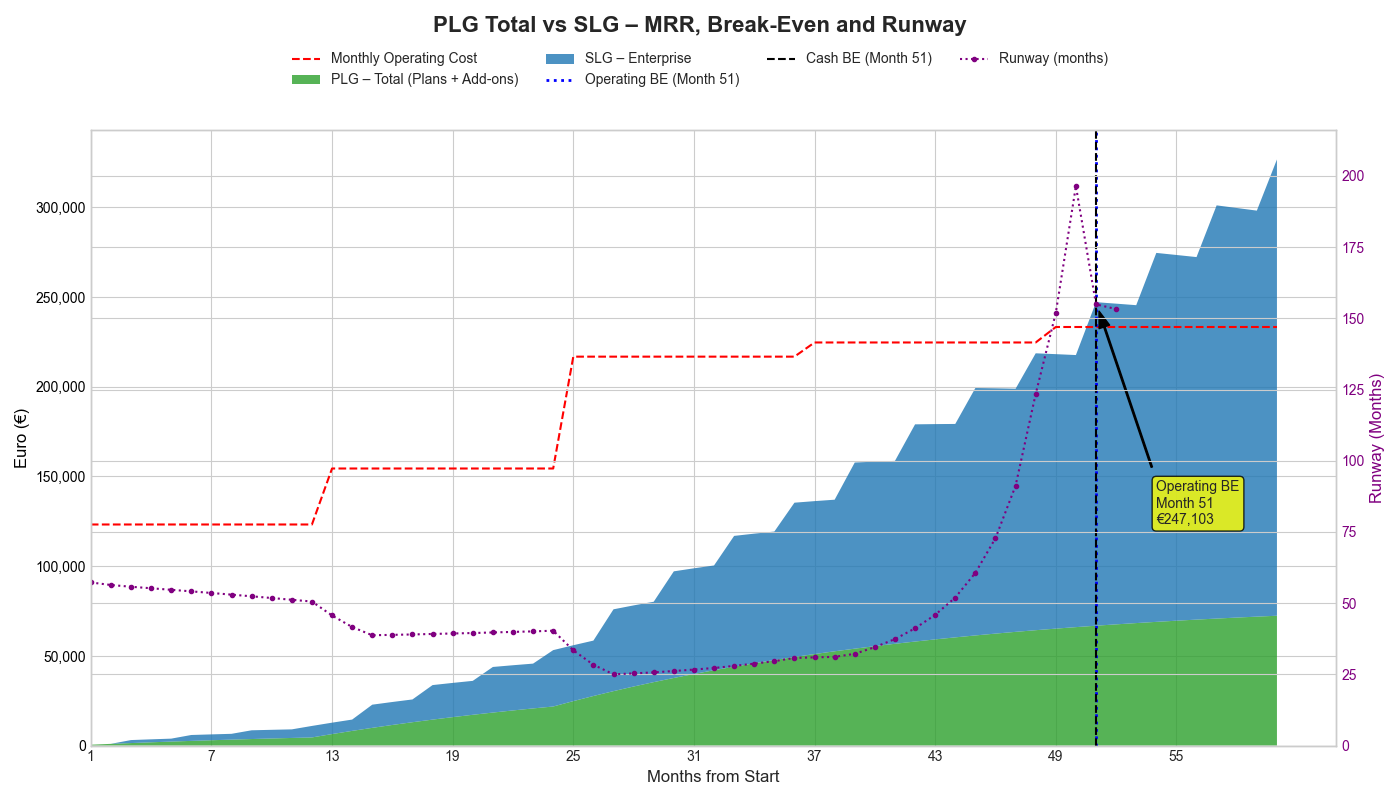
\includegraphics[width=\textwidth]{financial_projection.png}
    \caption{盈亏平衡分析:PLG 与 SLG 的 MRR、每月成本及跑道。}
    \label{fig:break_even_analysis}
\end{figure} 
\subsection{盈亏平衡分析:图表解读}

\paragraph{图例(快速阅读)}
\begin{itemize}
  \item \textbf{绿色(PLG -- 计划+附加组件):} 自助式经常性收入。
  \item \textbf{蓝色(SLG -- 企业):} 企业经常性收入;以季度“阶梯”增长,因为年度交易在季度间平滑。
  \item \textbf{红色虚线:} 每月运营成本(带谨慎调整上涨),按年度阶梯上升。
  \item \textbf{紫色点划线:} 运行时间(月数),计算方式为现金除以三个月移动平均燃烧。
  \item \textbf{垂直线:} 运营盈亏平衡点(蓝色,第51个月)和现金盈亏平衡点(黑色,第51个月)。
\end{itemize}

前三年图表展示了耐心构建的过程。绿色 PLG 区域随着月度注册(经调出后)持续增长,并且附加组件带来额外的MRR。蓝色 SLG 区域在企业合同时以明显的季度阶梯上升。成本块状变化:每一年新增计划容量(团队、基础设施、G\&A及其升降),因此红线跳跃后保持平坦,直到下一阶梯。

这些动态符合年终数字。第一年末:成本为 \textbf{€123,212}/月,而经常性MRR为 \textbf{€10,948}/月(亏损 \textbf{€112,149}/月),现金为 \textbf{€5,740,147},跑道为 \textbf{50.6} 个月。第二年:成本 \textbf{€154,413},MRR \textbf{€53,194}(亏损 \textbf{€100,855}/月),现金 \textbf{€4,282,549},跑道 \textbf{40.3} 个月。第三年:成本 \textbf{€216,746},MRR \textbf{€135,360}(亏损 \textbf{€80,631}/月),现金 \textbf{€2,239,361},跑道 \textbf{30.8} 个月。收入曲线明确缩小了与成本的差距,同时现金保持受控:观察到的最低跑道为 25.0 个月,峰值月燃烧为 \textbf{€160,442}。

到第四年,差距显著缩小。较大的 SLG 阶梯使蓝色区域扩展速度更快,PLG+SLG 堆叠几乎接近成本线。年末:成本 \textbf{€224,646}/月,MRR \textbf{€218,614}/月(总收入 \textbf{€219,615}/月),接近持平的亏损 \textbf{€5,031}/月,现金 \textbf{€2,239,361}。紫色跑道线开始剧烈上升,因为移动平均燃烧接近零。

% ----- End of translated content from: part_15.tex -----

% ----- Start of translated content from: part_16.tex -----

盈亏平衡点出现在 \textbf{第51个月}。在那时,\textbf{经常性月度经常性收入 (MRR) 为 €247{,}103},而成本为 \textbf{€233{,}271}(运营盈亏平衡点),且 \textbf{总收入 €248{,}159} 超过了成本(现金盈亏平衡点)。为了实现这一目标,模型累计 \textbf{消耗 €4{,}939{,}370},其中 \textbf{最低现金余额} 为 \textbf{€2{,}234{,}573},这也代表盈亏平衡时的 \textbf{储备(占融资轮的30.9\%)}。到第5年末,经常性MRR 达到 \textbf{€326{,}645}/月(约 \textbf{€3.92M ARR}),月利润为 \textbf{€94{,}565},现金余额为 \textbf{€2{,}673{,}539},且,财务跑道实际上变得无限长。

\paragraph{关键要点}
该图表清楚展示三点:
\begin{enumerate}
\item \emph{谁推动什么} PLG 构建基础,SLG 弥补差距
\item \emph{为何成本会上升} 有意的容量升级伴随审慎的增长策略
\item \emph{如何保障现金安全} 跑道从未崩溃(最少25.0个月),并随着收入超越成本而加快,就如所报告的指标所示。
\end{enumerate}

\begin{table}[H]
\centering
\caption{财务预测总结(年末)}
\label{tab:financial_summary}
\resizebox{\textwidth}{!}{
\begin{tabular}{lrrrrrrr}
\toprule
\textbf{年度末} & \textbf{月成本 (€)} & \textbf{经常性MRR (€)} & \textbf{存储收入 (€)} & \textbf{总收入 (€)} & \textbf{月亏盈 (€)} & \textbf{现金余额 (€)} & \textbf{跑道(月)} \\
\midrule
第1年 & 123,212 & 10,948 & 116 & 11,064 & -112,149 & 5,740,147 & 50.6 \\
第2年 & 154,413 & 53,194 & 364 & 53,558 & -100,855 & 4,282,549 & 40.3 \\
第3年 & 216,746 & 135,360 & 755 & 136,115 & -80,631 & 2,823,198 & 30.8 \\
第4年 & 224,646 & 218,614 & 1,001 & 219,615 & -5,031 & 2,239,361 & 123.5 \\
第5年 & 233,271 & 326,645 & 1,191 & 327,836 & 94,565 & 2,673,539 & 盈利 \\
\bottomrule
\end{tabular}
}
\end{table}

\begin{table}[H]
\centering
\caption{关键财务指标}
\label{tab:financial_metrics}
\resizebox{\textwidth}{!}{%
\begin{tabular}{ll}
\toprule
\textbf{指标} & \textbf{数值} \\
\midrule
运营盈亏平衡 & 第51个月(第5年):经常性MRR €247,103 $\geq$ 成本 €233,271 \\
盈亏平衡点 & 第51个月(第5年):总收入 €248,159 $\geq$ 成本 €233,271 \\
资本燃烧至现金盈亏平衡 & €4,939,370 \\
月最高燃烧 & €160,422 \\
期内最低现金余额 & €2,210,630(占轮次的30.9\%) \\
最短跑道(3个月移动平均) & 25.0个月 \\
\bottomrule
\end{tabular}
}
\end{table}

\newpage
\section{为何 CNY 59{,}829{,}055 是合理的金额}

我们请求 \textbf{CNY 59{,}829{,}055}(约 \textbf{€7.15M}),因为在我们的\emph{保守}场景中,这正是使公司在第51个月达到\textbf{运营及现金盈亏平衡}的资金量,而不会强制要求增长,同时保持一定的安全边际。模拟的结果明确:\textbf{累计燃烧至现金盈亏平衡}为 €4{,}939{,}370,\textbf{盈亏平衡时的现金余额}为 €2{,}210{,}630(即轮次的30.9\%),\textbf{路径中的最小跑道}为 25.0个月(3个月平均),而\textbf{月最高燃烧}为 €160{,}422。我们所请求的资金量是模型显示的实现盈亏平衡所需且充足的结构性缓冲。

这一计划设计得具有韧性:成本并非“裸简”,而是经过\textbf{类别性审慎提升}(基础设施、G\&A、PLG、SLG、R\&D、管理),以捕捉经常性项目(如企业支持、审计、法律、招聘、监控),这些常被低估。此外,模型引入了\textbf{自动保护机制}:如果跑道低于12个月,\textbf{下一月将裁减10\%的可选成本};低于9个月,则\textbf{付费PLG获取将减弱}(系数0.7)。这些都是编入模型的运营规则,不是承诺。实际上,风险由自动触发的机制保护。

在收入方面,我们明确区分\textbf{PLG}(计划+附加组件)和\textbf{SLG}(企业级)。这不是装饰性:它让我们可以逐月看到支出杠杆的回报,并实现无偏重的再平衡。利用此组合和当前价格,\textbf{运营盈亏平衡}在 \textbf{第51个月}实现,伴随着 \textbf{€247{,}103}的经常性MRR 与 \textbf{€233{,}271}的月成本;同期,\textbf{现金盈亏平衡}达成,因为\textbf{总收入 (€248{,}159)} 超过成本。到第5年末,经常性MRR 预计达到 \textbf{€326{,}645}(约 \textbf{€3.92M ARR})。从资本效率角度看,\textbf{隐性燃烧倍数}(燃烧至盈亏平衡除以盈亏平衡时的ARR)约为 \textbf{~1.66x},符合保守的产品+市场策略及合理的成本提升。

那么,为什么是这个额度而不是更少?因为少资本会导致模型更频繁触发保护机制,形成操作上的停顿与波动(裁减/冷却期),拉长时间表并增加机会成本,尤其在保持连续性最为关键时。为什么不更多?因为超过此阈值,瓶颈不在预算,而在\textbf{渠道吸收能力}和企业交付的自然节奏;多余的现金反而会增加稀释,而无法改善模型所示的结果。

\textbf{资金用途}仍紧扣模拟中的类别与提升:产品/R\&D(强化、可观测性、安全性)、基础设施与企业支持、SLG(账户、解决方案/验证)、PLG(内容/SDK/社区)、合作伙伴赋能、G\&A及合规、管理。我们不开新支出线,而是为模型已测算的项目提供资金。

最后,\textbf{风险画像}清晰:最低跑道不低于 \textbf{25.0个月},保护机制限制资金流失,在盈亏平衡点留存 \textbf{30.9\%} 缓冲,为应对采购延迟、基础设施或合规支出变动、外汇波动提供空间。同时,PLG/SLG的明确区分,使得资本配置能直观反映已实现的回报,而不是盲目套用统一模式。

\textbf{总结:} \textbf{CNY 59{,}829{,}055}完全覆盖保守路径的资金需求,具备充足的缓冲和自动成本控制。这是一份比例适当、合理、可复制的请求:投资者可以逐月验证模型指标的稳定性,确保现金流符合预期轨迹。

\subsection{战略缓冲理由:引领AI编排前沿}
盈亏平衡点的30.9\%资金储备(€2.21M)源自对AI编排市场前所未有的变革速度所做的深思熟虑的战略配置。不同于传统SaaS行业产品市场匹配规律,AI基础架构领域正经历每3-6个月一次的根本性变革——从新一代大模型架构到MCP等新兴编排标准。这一缓冲让IntellyHub能快速执行战略调整,无损跑道:无论是应对自主智能体能力的突破、整合在规划时尚未出现的变革模型,或是根据市场反馈在PLG与SLG渠道间调整焦点。这方面的成功AI基础架构公司(Weights \& Biases、Hugging Face)经验显示,赢者通常需经历2-3次重大转型,每次耗资占资本的15-20\%。我们的储备确保我们可以在保持12个月以上运营跑道的同时,执行一次重大策略调整,将潜在威胁转化为竞争优势。这并非多余资金,而是在一个唯一确定性为激进变革、比任何时刻都更快能调整的市场中,保险性质的策略性选择,确保在激烈的市场竞争中保持领先,避免被淘汰。

\newpage
\section{市场推广策略}
% 你将如何触达你的客户?

IntellyHub的市场进入策略采用混合模型,融合两大增长引擎:
\begin{enumerate}
    \item \textbf{以产品为导向的增长(PLG)—— SaaS:} 我们利用产品的优越性、免费层以及自动化商店,吸引、激活并在自下而上的基础上实现用户转化。
    \item \textbf{以销售为驱动的增长(SLG)—— 本地部署和企业端:} 我们采用针对性、咨询式的销售策略,赢取具有复杂安全与治理需求的大客户。
\end{enumerate}
这两种引擎相辅相成:PLG的成功为销售团队带来潜在客户和品牌认知,形成正反馈。

% ----- End of translated content from: part_16.tex -----

% ----- Start of translated content from: part_17.tex -----

% --- 战略目标 ---
\subsection{战略目标(3年展望)}
\begin{itemize}
    \item \textbf{定位:} 成为为现代技术团队策划复杂自动化和人工智能工作流的领先平台。
    \item \textbf{采纳:} 实现活跃用户数的临界规模,建立围绕插件生态系统和自动化商店的活跃社区。
    \item \textbf{收入:} 构建具有可持续性的商业模式,实现显著的年度经常性收入(ARR),既包括SaaS订阅,也包括企业本地合同。
\end{itemize}

% --- 第一年的目标 ---
\subsection{第一年:基础建设与市场验证}
\textbf{主要重点:} 赢得早期采用者,验证产品与市场的契合度,并获得首批关键参考客户(包括SaaS和本地部署客户)。在此阶段,许多活动是手动的,"不具规模"。

\newpage
\begin{table}[H]
\centering
\resizebox{\textwidth}{!}{
\begin{tabularx}{\textwidth}{L L L} 
\toprule
\textbf{关键渠道} & \textbf{具体行动} & \textbf{成功关键指标} \\

\midrule
\textbf{产品驱动增长 (PLG)} & 
\textbf{细分市场发布:} 在Product Hunt、Hacker News以及相关技术子版块(如 r/devops、r/kubernetes)上展示IntellyHub。\newline\newline
\textbf{自动化商店:} 充实商店,提供20-30个高质量的官方模板,解决实际且痛苦的问题。
&
\textbf{激活率:} >25\%(用户在7天内运行他们的第一个自动化)。\newline\newline
\textbf{一个月留存:} >15\%(用户四周后回访)。
\\
\addlinespace

\textbf{技术内容营销} & 
\textbf{博客与教程:} 每月发布2-4篇深入的技术文章,展示如何用IntellyHub解决具体问题。\newline\newline
\textbf{视频内容:} 制作简洁明了的视频教程。
&
\textbf{合格流量:} 来自自然搜索和推荐渠道的访问量。\newline\newline
\textbf{访客转注册率:} >2\%。
\\
\addlinespace

\textbf{社区建设} &
\textbf{Discord/Slack频道:} 建立早期用户的交流中心。\newline\newline
\textbf{由创始人领导的支持:} 亲自回复每个问题和反馈请求,以建立良好的关系。
&
\textbf{社区活跃度:} 每周活跃成员数,同行支持互动。\newline\newline
\textbf{定性反馈:} 每月不少于5次深入用户访谈。
\\
\addlinespace

\textbf{由创始人带领的销售(本地部署)} &
\textbf{利用网络:} 创始人通过自己的网络,亲自管理前3-5个目标公司销售流程。\newline\newline
\textbf{概念验证(POC):} 集中于少数高价值的POC成功。
&
\textbf{启动POC数:} 年内完成3-5个。\newline\newline
\textbf{签署本地部署合同:} 1-2个关键参考客户。
\\
\bottomrule
\end{tabularx}
}
\end{table}

% --- 第二年的目标 ---
\newpage
\subsection{第二年:扩展与构建可重复的增长引擎}
\textbf{主要重点:} 将初步价值转化为可扩展、可重复的流程。优化第一年中行之有效的方法,并建立一支商业团队的基础。

\begin{table}[H]
\small
\centering
\resizebox{\textwidth}{!}{
\begin{tabularx}{\textwidth}{L L L}
\toprule
\textbf{关键渠道} & \textbf{具体行动} & \textbf{成功关键指标} \\
\midrule
\textbf{PLG优化} &

\textbf{漏斗分析:} 使用分析工具识别并消除用户从注册到付费转化过程中的摩擦点。
\textbf{引导式入门:} 实现应用内引导,帮助新用户找到“灵感时刻”。
&

% ----- End of translated content from: part_17.tex -----

% ----- Start of translated content from: part_18.tex -----

\textbf{免费转付费转化率:} >3\%。\textbf{月度经常性收入(MRR)增长率:} 持续逐月增长。\\
\addlinespace
\textbf{生态系统合作伙伴关系} &

\textbf{战略集成:} 积极开发2-3个具有类似用户群的互补技术平台的插件。\textbf{共同营销:} 与合作伙伴一同启动联合营销活动(网络研讨会、博客文章)。&

\textbf{合作伙伴引荐线索。}
\textbf{合作插件下载量。}
\\
\addlinespace
\textbf{初始销售团队} &

\textbf{首批招聘:} 增聘另一名客户经理,以处理内线线索并开始目标外呼潜在客户。\textbf{销售手册:} 根据创始人带领销售阶段的经验教训,将销售流程制度化。&

\textbf{每月合格演示次数。}
\textbf{平均销售周期(本地部署)。}
\\
\bottomrule
\end{tabularx}
}
\end{table}

\newpage
% --- 第三年 ---
\subsection{第3年:扩大规模与细分市场领导力}
\textbf{主要关注点:} 加速增长,主导技术团队细分市场,建立IntellyHub在AI编排市场中的思想领导地位。

\begin{table}[H]
\centering
\resizebox{\textwidth}{!}{
\begin{tabularx}{\textwidth}{L L L}
\toprule
\textbf{主要渠道} & \textbf{具体措施} & \textbf{成功关键绩效指标(KPIs)} \\
\midrule
\textbf{销售扩展性} &

\textbf{团队扩充:} 拓展销售团队覆盖不同地区或行业垂直市场。\textbf{间接渠道:} 开始探索与系统集成商和经销商的合作伙伴关系。 &

\textbf{年度经常性收入(ARR)增长。}
\textbf{客户获取成本(CAC)与客户终身价值/CAC比率。}
\\
\addlinespace
\textbf{品牌营销} &

\textbf{思想领导:} 发布基于平台数据的行业报告。\textbf{赞助活动:} 赞助在DevOps和AI领域的关键会议和播客。&

\textbf{行业媒体提及。}
\textbf{直接与品牌流量增长。}
\\
\addlinespace
\textbf{网络效应} &

\textbf{开放商店:} 开放自动化商店和插件市场,接受外部贡献证书合作伙伴。\textbf{开发者计划:} 推出正式的开发者关系(DevRel)项目。&

\textbf{社区创建的插件/模板数量。}
\textbf{净收入留存(NRR):} >110\%。\\
\bottomrule
\end{tabularx}
}
\end{table}

\clearpage
\section{运营计划}
% 公司的日常运作将如何进行。
\subsection{介绍}
本文档概述了执行IntellyHub开发和市场推广战略的运营计划。该计划与产品开发路线图的各阶段保持一致,描述了公司各职能领域的关键活动。

% ----- End of translated content from: part_18.tex -----

% ----- Start of translated content from: part_19.tex -----

% --- 阶段 1 ---
\subsection{阶段 1:基础与验证(第1-2季度)}
\textbf{战略目标:} 将原型转变为稳定且安全的 MVP,获取首批早期采用者,并 \textbf{通过有针对性的合作伙伴计划验证核心产品和定价模型假设。}

\subsubsection{产品开发与工程}
\begin{itemize}[leftmargin=*]
    \item \textbf{第1季度:}
    \begin{itemize}
        \item \textbf{稳定性:} 完成测试套件(单元测试、集成测试),确保核心引擎的可靠性。
        \item \textbf{插件:} 完成并记录内部系统,以实现标准化插件开发。
        \item \textbf{UI/UX:} 优化混合 IDE 界面,解决同步问题并提升用户体验。
        \item \textbf{本地部署:} 开发并测试企业客户的本地版平台。
    \end{itemize}
    \item \textbf{第2季度:}
    \begin{itemize}
        \item \textbf{身份验证:} 实现健壮的用户管理与身份验证系统。
        \item \textbf{引导流程:} 开发新用户的引导向导。
        \item \textbf{商店(v1):} 创建自动化商店第一版的 API 和界面(只读模式)。
    \end{itemize}
\end{itemize}

\subsubsection{市场推广(营销与销售)}
\begin{itemize}[leftmargin=*]
    \item \textbf{第1-2季度:}
    \begin{itemize}
        \item \textbf{垂直行业策略:} 在\textit{最初的垂直行业细分}(例如基于 Esplorado 用户案例的 BioTech/科研)内定义详细的理想客户画像(ICP)。
        \item \textbf{(新)设计合作伙伴计划:} 推出针对目标行业内3-5家精选公司的独家计划,提供早期访问和直接支持,以换取持续反馈和潜在的初步合同。
    \end{itemize}
    \item \textbf{第3-4季度:}
    \begin{itemize}
        \item \textbf{特定市场推广:} 在 Product Hunt、Hacker News 和相关渠道启动,强调所选行业的特色。
        \item \textbf{反馈收集:} 收集来自免费层用户和优先关注的设计合作伙伴的结构化反馈。
    \end{itemize}
\end{itemize}

\subsubsection{社区 \& 生态系统管理}
\begin{itemize}[leftmargin=*]
    \item \textbf{第1-2季度:}
    \begin{itemize}
        \item \textbf{定向插件开发:} 开发并记录首批“官方”插件,\textit{优先开发与目标行业最相关的插件}。
    \end{itemize}
    \item \textbf{第3-4季度:}
    \begin{itemize}
        \item \textbf{社区建设:} 推出官方 Discord/Slack 服务器。
        \item \textbf{参与互动:} 创始人和开发团队将积极参与,解答问题,营造友好氛围。
    \end{itemize}
\end{itemize}

\subsubsection{普通及企业运营}
\begin{itemize}[leftmargin=*]
    \item \textbf{第1-2季度:}
    \begin{itemize}
        \item \textbf{法律与行政准备:} 最终确定公司结构,开设银行账户。
        \item \textbf{(新)合作协议:} 准备“设计合作伙伴计划”的协议文件。
    \end{itemize}
    \item \textbf{第3-4季度:}
    \begin{itemize}
        \item \textbf{服务条款制定:} 编写并公布免费层的服务条款和隐私政策。
    \end{itemize}
\end{itemize}

\clearpage

% --- 阶段 2 ---
\subsection{阶段 2:扩展与增长(第3-4季度)}
\textbf{战略目标:} 在第1阶段验证数据基础上,扩大用户获取,拓展生态系统,并实现必要的企业功能以实现盈利。

\subsubsection{产品开发与工程}
\begin{itemize}[leftmargin=*]
    \item \textbf{第5-6季度:}
    \begin{itemize}
        \item \textbf{安全性:} 实现密钥管理系统以保护凭据。
        \item \textbf{版本控制:} 添加自动化的历史记录与回滚功能。
    \end{itemize}
    \item \textbf{第7-8季度:}
    \begin{itemize}
        \item \textbf{可观察性:} 开发数据平台的首个版本,用于流性能指标的监控。
        \item \textbf{改进仪表盘:} 创建用于可视化工作流的用户界面。
        \item \textbf{主动AI:} 实现基于流性能数据的基础“自动修复”功能。

% ----- End of translated content from: part_19.tex -----

% ----- Start of translated content from: part_20.tex -----

\end{itemize}
\end{itemize}

\subsubsection{Go-to-Market(市场营销与销售)}
\begin{itemize}[leftmargin=*]
    \item \textbf{Q5-Q6:}
    \begin{itemize}
        \item \textbf{垂直内容营销:} 扩大针对所选垂直领域的内容(案例研究基于Design Partners,文章)的生产规模。
        \item \textbf{招聘:} 开始招聘第一位开发者大使。
    \end{itemize}
    \item \textbf{Q7-Q8:}
    \begin{itemize}
        \item \textbf{付费套餐发布:} 最终确定定价(经过Design Partners验证)并正式推出Pro和Enterprise计划。
        \item \textbf{销售手册(v1):} 开始整理企业客户的销售流程。
    \end{itemize}
\end{itemize}

\clearpage

% --- PHASE 3 ---
\section{第三阶段:领导力与创新(第5-6季度)}
\textbf{战略目标:} 建立市场领导地位,通过社区创造网络效应,并**利用数据建立难以超越的竞争优势。**

\subsubsection{产品开发与工程}
\begin{itemize}[leftmargin=*]
    \item \textbf{Q9-Q10:}
    \begin{itemize}
        \item \textbf{开店:} 开放商店,允许社区成员提交内容。
        \item \textbf{内容审核:} 实施内部工具以审查和验证外部贡献。
    \end{itemize}
    \item \textbf{Q11-Q12:}
    \begin{itemize}
        \item \textbf{(修订版)数据平台与可观察性:} 开发收集和聚合流量性能指标的系统,战略目标是 \textbf{构建“数据护城河”}。
        \item \textbf{分析仪表盘:} 创建可视化分析的用户界面。
        \item \textbf{主动型AI:} 改善“自动修复”和主动优化功能,\textbf{基于聚合平台数据进行训练}。
    \end{itemize}
\end{itemize}

\subsubsection{市场推广(营销与销售)}
\begin{itemize}[leftmargin=*]
    \item \textbf{Q9-Q10:}
    \begin{itemize}
        \item \textbf{销售团队扩展:} 招聘额外的客户执行员以覆盖特定市场或垂直领域。
        \item \textbf{行业领袖:} 开始发布基于平台使用数据的报告和分析。
    \end{itemize}
    \item \textbf{Q11-Q12:}
    \begin{itemize}
        \item \textbf{品牌营销:} 增加品牌知名度活动的投入(赞助、活动)。
    \end{itemize}
\end{itemize}

\newpage
\section{风险分析}
\subsection{市场风险}
\textit{与市场、竞争和客户采纳相关的风险。}

\begin{table}[H]
\centering
\begin{tabularx}{\textwidth}{@{}lL@{}}
\toprule
\textbf{风险} & \textbf{描述} \\
\midrule
\textbf{来自“现状”的竞争} & 我们最大的竞争对手不是另一个平台,而是开发者使用自定义Python脚本的惯性。它们的熟悉程度和零初期成本的感知成为重大障碍。 \\
\addlinespace
\textbf{企业级采用缓慢周期} & 内部部署和企业销售模型对于高价值合同至关重要,但其特征是销售周期长(6-12个月以上)且包含复杂的概念验证(POC)阶段。第一批关键企业交易的延迟可能会严重影响收入预测。 \\
\addlinespace
\textbf{AI技术转变} & 我们的AI目前定位为“协同驾驶员”。竞争对手若迅速在技术上跨越,开发出真正自治且“足够好”的AI代理,可能会让我们较受控、结构化的方法变得不那么创新。 \\
\bottomrule
\end{tabularx}
\end{table}

\newpage
\subsection{运营风险}
\textit{与技术、人事和执行相关的风险。}

\begin{table}[H]
\centering
\begin{tabularx}{\textwidth}{@{}lL@{}}
\toprule
\textbf{风险} & \textbf{描述} \\

% ----- End of translated content from: part_20.tex -----

% ----- Start of translated content from: part_21.tex -----

\midrule
\textbf{团队执行与关键人员风险} & 该计划依赖于招聘少数高度专业化的人员。项目的成功在很大程度上取决于核心团队在产品、基础设施和销售方面的执行能力。关键成员的离职可能会导致重大延误。 \\
\addlinespace
\textbf{技术复杂性} & 技术栈(Kubernetes、多步骤AI管道、混合IDE)具有极强的功能,但维护和演进也同样复杂。在该复杂系统中出现的漏洞、安全漏洞或性能瓶颈难以解决且成本高昂。 \\
\addlinespace
\textbf{混合技术风险(IDE/YAML同步)} & 在复杂的视觉IDE与文本YAML表示之间保持完美、实时的双向同步在技术方面具有挑战性。这可能成为微妙且难以调试的Bug源,影响用户信任。 \\
\addlinespace
\textbf{生态系统质量控制} & 自动化商店(Automation Store)和插件市场(Plugin Marketplace)的价值犹如双刃剑。低质量、不安全或维护不善的社区贡献可能损害用户信任和平台声誉。 \\
\bottomrule
\end{tabularx}
\end{table}

\newpage
\subsection{财务风险}
\textit{与现金流、资金和财务可持续性相关的风险。}

\begin{table}[H]
\centering
\begin{tabularx}{\textwidth}{@{}lL@{}}
\toprule
\textbf{风险} & \textbf{描述} \\
\midrule
\textbf{高初始烧钱率} & 积极的招聘计划导致在实现显著收入之前每月运营成本很高。这对快速达到产品市场匹配和产生收入施加巨大压力。 \\
\addlinespace
\textbf{资金依赖} & 商业模式并未为短期盈利设计。不达预期的增长KPI可能成为生存威胁。 \\
\addlinespace
\textbf{定价模型验证} & 提议的价值指标(执行次数、活跃自动化数)逻辑合理,但未经验证。定价模型不正确可能导致客户不满(价格过高)或大量潜在收入流失(价格过低)。 \\
\bottomrule
\end{tabularx}
\end{table}

\newpage
\subsection{缓解策略}
\textit{针对已识别风险的具体行动方案。}

\begin{table}[H]
\centering
\begin{tabularx}{\textwidth}{@{}lL@{}}
\toprule
\textbf{风险类别} & \textbf{缓解策略} \\
\midrule
\textbf{市场风险} & 
\textbf{定位与教育:} 将市场推广的重点放在消除“管理许多脚本”的长期混乱上,而非取代单一脚本。利用“Esplorado”等案例研究,提供无可争辩的价值证明。 \newline\newline
\textbf{混合GTM:} 同步推进PLG(SaaS)和SLG(本地部署)策略。利用PLG快速反馈环完善产品和信息传递,以支持较慢的企业销售周期。 \newline\newline
\textbf{战略性AI路线图:} 将当前AI定位为生产环境中务实、安全、可靠的选择。将路线图描述为朝更自主能力发展的演进,建立在我们今天坚实的基础之上。 \\
\addlinespace
\textbf{运营风险} & 
\textbf{文档与交叉培训:} 从一开始就大量投入内部文档,建立知识共享和配对编程文化,以减少对单一人员的依赖。 \newline\newline
\textbf{投资于可观察性与测试:} 配备强大的自动化测试套件,尽早集成APM(应用性能监控)工具,以主动定位和解决问题。测试套件特别覆盖IDE/YAML同步逻辑。 \newline\newline
\textbf{精选生态系统:} 初期仅提供“官方”和“认证合作伙伴”插件。对未来社区提交实行明确、严格的审查流程,包括自动安全扫描和质量检测。 \\
\addlinespace
\textbf{财务风险} & 
\textbf{里程碑驱动支出:} 将主要支出增加(尤其是市场营销和销售招聘)与达成具体、预定义的里程碑挂钩(如首批10个付费客户、达成某个留存率)。 \newline\newline
\textbf{持续投资者关系:} 保持与现有及潜在未来投资者的透明、定期沟通,分享关键绩效指标(KPIs),以增强信心并简化下一轮融资筹备。 \newline\newline
\textbf{定价迭代:} 采用简单且灵活的价格模型进行初步推出。直接与早期客户沟通,了解他们的价值感知,并根据反馈和使用数据准备迭代定价结构。 \\
\bottomrule
\end{tabularx}
\end{table}

% ----- End of translated content from: part_21.tex -----

% ----- Start of translated content from: part_22.tex -----
\begin{thebibliography}{99}
    \bibitem{AIMarket}
    Market.us, \textit{Automated Machine Learning Market Report}, Available at: \url{https://market.us/report/automated-machine-learning-market/}, March~2025.
    
    \bibitem{MLOpsMarket}
    MarketReserchFuture.com, \textit{Mlops Market Research Report: Information By Component (Service, Platform), By Deployment Mode (On-Premises, Cloud), By Organization Size (Large Enterprise, SME's), By Verticals (BFSI, Retail and e-Commerce, Government and Defense, Healthcare and Life science, Manufacturing, and Others) And By Region (North America, Europe, Asia-Pacific, And Rest Of The World) –Market Forecast Till 2034.}, Available at: \url{https://www.marketresearchfuture.com/reports/mlops-market-18849}, Agoust~2025.
    
    \bibitem{AIOrch}
    Market.us, \textit{AI Orchestration Platform Market Report (2024--2034 Forecast)}, February~2025.  
    Available at: \url{https://market.us/report/ai-orchestration-platform-market/}.

    \bibitem{GartnerAgentic}
    Reuters (reporting Gartner), \textit{Over 40\% of agentic AI projects will be scrapped by 2027 … by 2028, 33\% of enterprise software will include agentic AI and 15\% of decisions will be made autonomously,} June~25,~2025.  
    Available at: \url{https://www.reuters.com/business/over-40-agentic-ai-projects-will-be-scrapped-by-2027-gartner-says-2025-06-25/}.

    \bibitem{MLOpsMM}
    MarketsandMarkets Research, \textit{MLOps Market Size is Anticipated to Cross US\$5.9 Billion by 2027, growing at a CAGR of 41.0\%}, April~21,~2023.  
    Available at: \url{https://www.globenewswire.com/news-release/2023/04/21/2652028/0/en/MLOps-Market-Size-is-Anticipated-to-Cross-US-5-9-billion-by-2027-growing-at-a-CAGR-of-41-0-Report-by-MarketsandMarkets.html}.

    \bibitem{ModelOpsGV}
    Grand View Research, \textit{ModelOps Market Report}, 2025 edition.  
    Available at: \url{https://www.grandviewresearch.com/industry-analysis/modelops-market-report}.

    \bibitem{AIMLMarket}
    Market.us, \textit{Automated Machine Learning Market Report (2024--2034 Forecast)}, March~2025.  
    Available at: \url{https://market.us/report/automated-machine-learning-market/}.

    \bibitem{MLOpsMM}
    MarketsandMarkets Research,\textit{MLOps市场规模预计到2027年将突破59亿美元,年复合增长率为41.0\%},2023年4月21日。
    网址:\url{https://www.globenewswire.com/news-release/2023/04/21/2652028/0/en/MLOps-Market-Size-is-Anticipated-to-Cross-US-5-9-billion-by-2027-growing-at-a-CAGR-of-41-0-Report-by-MarketsandMarkets.html}。

    \bibitem{ModelOpsGV}
    Grand View Research,\textit{ModelOps市场报告},2025版。
    网址:\url{https://www.grandviewresearch.com/industry-analysis/modelops-market-report}。

    \bibitem{AIMLMarket}
    Market.us,\textit{自动化机器学习市场报告(2024--2034预测)},2025年3月。
    网址:\url{https://market.us/report/automated-machine-learning-market/}。

    \bibitem{MLOpsMRF}
    MarketResearchFuture,\textit{MLOps市场研究报告(2024--2034预测)},2025年8月。
    网址:\url{https://www.marketresearchfuture.com/reports/mlops-market-18849}。

    \bibitem{deloitte2020}
    Deloitte,\textit{智能边缘自动化:企业新前沿},2020年。网址:\url{https://www2.deloitte.com/us/en/insights/topics/talent/intelligent-automation-2020-survey-results.html}

    \bibitem{grandviewRPA}
    Grand View Research,\textit{机器人流程自动化(RPA)市场规模、份额与趋势分析报告},2024年。
    网址:\url{https://www.grandviewresearch.com/industry-analysis/robotic-process-automation-rpa-market}

    \bibitem{mckinseyAI2023}
    McKinsey \& Company,\textit{2023年AI现状:生成式AI的爆发之年},2023年8月1日。
    网址:\url{https://www.mckinsey.com/capabilities/quantumblack/our-insights/the-state-of-ai-in-2023-generative-ais-breakout-year}

    \bibitem{langchainGitHub}
    LangChain GitHub仓库。网址:\url{https://github.com/langchain-ai/langchain}

    \bibitem{gartnerAIBarriers}
    Gartner,\textit{AI采纳的两个障碍},2021年11月2日。
    网址:\url{https://www.gartner.com/en/articles/2-barriers-to-ai-adoption}

    \bibitem{euAIAct}
    欧盟委员会,\textit{人工智能监管框架提案}。
    网址:\url{https://digital-strategy.ec.europa.eu/en/policies/regulatory-framework-ai}

    \bibitem{AIOrch}
    Market.us,\textit{AI调度平台市场报告(2024--2034预测)},2025年2月。
    网址:\url{https://market.us/report/ai-orchestration-platform-market/}。

    \bibitem{zapierApps}
    Zapier,\textit{探索6000多个应用}。网址:\url{https://zapier.com/apps}

    \bibitem{g2ZapierReviews}
    G2,\textit{Zapier评价}。网址:\url{https://www.g2.com/products/zapier/reviews}

    \bibitem{zapierPricing}
    Zapier,\textit{Zapier定价方案}。网址:\url{https://zapier.com/pricing}

    \bibitem{zapierOpenAI}
    Zapier,\textit{OpenAI集成}。网址:\url{https://zapier.com/apps/openai/integrations}

    \bibitem{g2MakeVsZapier}
    G2,\textit{比较Make与Zapier}。网址:\url{https://www.g2.com/compare/make-vs-zapier}

    \bibitem{autogenGitHub}
    Microsoft,\textit{AutoGen GitHub仓库}。网址:\url{https://github.com/microsoft/autogen}

    \bibitem{crewaiGitHub}
    Joao Moura,\textit{CrewAI GitHub仓库}。网址:\url{https://github.com/joaomdmoura/crewAI}

    \bibitem{langchainValuation}
    TechCrunch,\textit{AI基础设施初创公司LangChain据报道融资1亿美元,估值11亿美元},2025年7月9日。
    网址:\url{https://siliconangle.com/2025/07/09/ai-infrastructure-startup-langchain-reportedly-raises-100m-1-1b-valuation/#:~:text=Artificial%20intelligence%20infrastructure%2C%20developer%20tools,on%20a%20%241.1%20billion%20valuation.}

    \bibitem{langchainIntegrations}
    LangChain文档,\textit{LangChain集成}。网址:\url{https://python.langchain.com/docs/integrations/providers/}

    \bibitem{langchainCritique}
    Medium,\textit{LangChain的挑战与批评},2025年3月3日。
    网址:\url{https://shashankguda.medium.com/challenges-criticisms-of-langchain-b26afcef94e7}

    \bibitem{mrfRPA}
    Market Research Future,\textit{机器人流程自动化(RPA)市场研究报告信息,包括流程(决策支持、自动化解决方案和管理方案)、操作(规则基础和知识基础)、行业(制造业与物流、信息技术与电信)及地区(北美、欧洲、亚太及其他地区)——行业规模、份额及至2032年的预测}。
    网址:\url{https://www.marketresearchfuture.com/reports/robotic-process-automation-market-2209}

    \bibitem{uipathGartner}
    UiPath,\textit{Gartner RPA魔力象限},2025年。
    网址:\url{https://www.uipath.com/resources/automation-analyst-reports/gartner-magic-quadrant-robotic-process-automation}

    \bibitem{awsSagemaker}
    亚马逊AWS SageMaker,\textit{亚马逊SageMaker}。
    网址:\url{https://aws.amazon.com/sagemaker/}

    \bibitem{forresterRPAvsAI}
    Craig Le Clair, \textit{RPA平台会保持相关性吗?AI代理可能是答案。}, Forrester, 2024年4月25日。 访问地址:\url{https://www.forrester.com/blogs/will-rpa-platforms-remain-relevant-ai-agents-may-hold-the-answer/}

\end{thebibliography}


\end{document}

